% Options for packages loaded elsewhere
\PassOptionsToPackage{unicode}{hyperref}
\PassOptionsToPackage{hyphens}{url}
\PassOptionsToPackage{dvipsnames,svgnames,x11names}{xcolor}
%
\documentclass[
  letterpaper,
  DIV=11,
  numbers=noendperiod]{scrreprt}

\usepackage{amsmath,amssymb}
\usepackage{lmodern}
\usepackage{iftex}
\ifPDFTeX
  \usepackage[T1]{fontenc}
  \usepackage[utf8]{inputenc}
  \usepackage{textcomp} % provide euro and other symbols
\else % if luatex or xetex
  \usepackage{unicode-math}
  \defaultfontfeatures{Scale=MatchLowercase}
  \defaultfontfeatures[\rmfamily]{Ligatures=TeX,Scale=1}
\fi
% Use upquote if available, for straight quotes in verbatim environments
\IfFileExists{upquote.sty}{\usepackage{upquote}}{}
\IfFileExists{microtype.sty}{% use microtype if available
  \usepackage[]{microtype}
  \UseMicrotypeSet[protrusion]{basicmath} % disable protrusion for tt fonts
}{}
\makeatletter
\@ifundefined{KOMAClassName}{% if non-KOMA class
  \IfFileExists{parskip.sty}{%
    \usepackage{parskip}
  }{% else
    \setlength{\parindent}{0pt}
    \setlength{\parskip}{6pt plus 2pt minus 1pt}}
}{% if KOMA class
  \KOMAoptions{parskip=half}}
\makeatother
\usepackage{xcolor}
\usepackage[normalem]{ulem}
\setlength{\emergencystretch}{3em} % prevent overfull lines
\setcounter{secnumdepth}{5}
% Make \paragraph and \subparagraph free-standing
\ifx\paragraph\undefined\else
  \let\oldparagraph\paragraph
  \renewcommand{\paragraph}[1]{\oldparagraph{#1}\mbox{}}
\fi
\ifx\subparagraph\undefined\else
  \let\oldsubparagraph\subparagraph
  \renewcommand{\subparagraph}[1]{\oldsubparagraph{#1}\mbox{}}
\fi


\providecommand{\tightlist}{%
  \setlength{\itemsep}{0pt}\setlength{\parskip}{0pt}}\usepackage{longtable,booktabs,array}
\usepackage{calc} % for calculating minipage widths
% Correct order of tables after \paragraph or \subparagraph
\usepackage{etoolbox}
\makeatletter
\patchcmd\longtable{\par}{\if@noskipsec\mbox{}\fi\par}{}{}
\makeatother
% Allow footnotes in longtable head/foot
\IfFileExists{footnotehyper.sty}{\usepackage{footnotehyper}}{\usepackage{footnote}}
\makesavenoteenv{longtable}
\usepackage{graphicx}
\makeatletter
\def\maxwidth{\ifdim\Gin@nat@width>\linewidth\linewidth\else\Gin@nat@width\fi}
\def\maxheight{\ifdim\Gin@nat@height>\textheight\textheight\else\Gin@nat@height\fi}
\makeatother
% Scale images if necessary, so that they will not overflow the page
% margins by default, and it is still possible to overwrite the defaults
% using explicit options in \includegraphics[width, height, ...]{}
\setkeys{Gin}{width=\maxwidth,height=\maxheight,keepaspectratio}
% Set default figure placement to htbp
\makeatletter
\def\fps@figure{htbp}
\makeatother

\KOMAoption{captions}{tableheading}
\makeatletter
\makeatother
\makeatletter
\@ifpackageloaded{bookmark}{}{\usepackage{bookmark}}
\makeatother
\makeatletter
\@ifpackageloaded{caption}{}{\usepackage{caption}}
\AtBeginDocument{%
\ifdefined\contentsname
  \renewcommand*\contentsname{Table of contents}
\else
  \newcommand\contentsname{Table of contents}
\fi
\ifdefined\listfigurename
  \renewcommand*\listfigurename{List of Figures}
\else
  \newcommand\listfigurename{List of Figures}
\fi
\ifdefined\listtablename
  \renewcommand*\listtablename{List of Tables}
\else
  \newcommand\listtablename{List of Tables}
\fi
\ifdefined\figurename
  \renewcommand*\figurename{Figure}
\else
  \newcommand\figurename{Figure}
\fi
\ifdefined\tablename
  \renewcommand*\tablename{Table}
\else
  \newcommand\tablename{Table}
\fi
}
\@ifpackageloaded{float}{}{\usepackage{float}}
\floatstyle{ruled}
\@ifundefined{c@chapter}{\newfloat{codelisting}{h}{lop}}{\newfloat{codelisting}{h}{lop}[chapter]}
\floatname{codelisting}{Listing}
\newcommand*\listoflistings{\listof{codelisting}{List of Listings}}
\makeatother
\makeatletter
\@ifpackageloaded{caption}{}{\usepackage{caption}}
\@ifpackageloaded{subcaption}{}{\usepackage{subcaption}}
\makeatother
\makeatletter
\@ifpackageloaded{tcolorbox}{}{\usepackage[many]{tcolorbox}}
\makeatother
\makeatletter
\@ifundefined{shadecolor}{\definecolor{shadecolor}{rgb}{.97, .97, .97}}
\makeatother
\makeatletter
\makeatother
\ifLuaTeX
  \usepackage{selnolig}  % disable illegal ligatures
\fi
\IfFileExists{bookmark.sty}{\usepackage{bookmark}}{\usepackage{hyperref}}
\IfFileExists{xurl.sty}{\usepackage{xurl}}{} % add URL line breaks if available
\urlstyle{same} % disable monospaced font for URLs
\hypersetup{
  colorlinks=true,
  linkcolor={blue},
  filecolor={Maroon},
  citecolor={Blue},
  urlcolor={Blue},
  pdfcreator={LaTeX via pandoc}}

\author{}
\date{}

\begin{document}
\ifdefined\Shaded\renewenvironment{Shaded}{\begin{tcolorbox}[interior hidden, frame hidden, enhanced, boxrule=0pt, sharp corners, borderline west={3pt}{0pt}{shadecolor}, breakable]}{\end{tcolorbox}}\fi

\renewcommand*\contentsname{Table of contents}
{
\hypersetup{linkcolor=}
\setcounter{tocdepth}{2}
\tableofcontents
}
\bookmarksetup{startatroot}

\hypertarget{livret-des-stages}{%
\chapter{\texorpdfstring{\textbf{Livret des
stages}}{Livret des stages}}\label{livret-des-stages}}

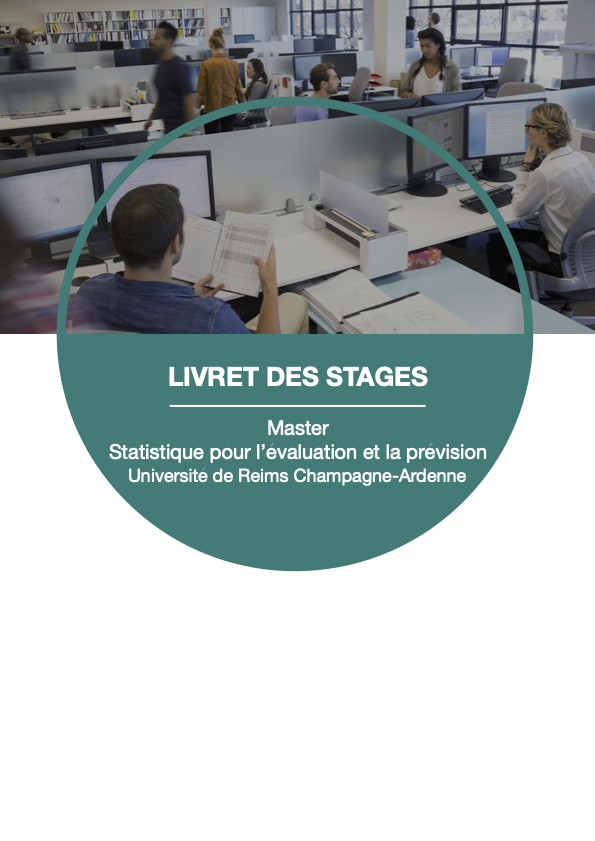
\includegraphics{./images/page.png}

\bookmarksetup{startatroot}

\hypertarget{pruxe9sentation-du-master-sep}{%
\chapter{Présentation du master
SEP}\label{pruxe9sentation-du-master-sep}}

Le Master 2 Statistique pour l'Évaluation et la Prévision (SEP) forme
des statisticiens compétents et polyvalents, capables d'intervenir dans
des domaines très variés. Il vise principalement deux objectifs : un
objectif de savoir-faire qui consiste à procurer aux étudiants des
compétencestechniques et un objectif de polyvalence qui va leur
permettre d'intégrer et de travailler au sein de toute structure dotée
d'un service statistique et impliquant des interactions avec d'autres
disciplines.

Une des spécificités de la formation est de confronter tout au long de
l'année les étudiants à la pluridisciplinarité, ce qui permettra à ces
derniers d'être capables de tenir un discours intelligible dans tous les
domaines où les statistiques sont présentes

La formation des étudiants du master 2 se fait à travers des modules de
cours bien définis dont on citera :

\begin{itemize}
\item
  L'analyse des systèmes complexes : L'analyse décisionnelle des
  systèmes complexes est une discipline qui vise à fournir des méthodes
  et outils de pilotage des systèmes complexes ou de modélisation des
  environnements chaotiques (théorie du chaos). La démarche insiste sur
  la transdisciplinarité et inscrit donc l'Analyse décisionnelle des
  systèmes complexes dans le courant de pensée systémique
\item
  L'apprentissage automatique : L'apprentissage automatique ou
  apprentissage statistique est un champ d'étude de l'intelligence
  artificielle qui se base sur des approches statistiques pour donner
  aux ordinateurs la capacité d'« apprendre » à partir de données,
  c'est-à-dire d'améliorer leurs performances à résoudre des tâches sans
  être explicitement programmés pour chacune. Plus largement, cela
  concerne la conception, l'analyse, le développement et
  l'implémentation de telles méthodes
\item
  Les outils Big Data : Les bases de données relationnelles classiques
  ne permettent pas de gérer les volumes de données du big data. De
  nouveaux modèles de représentation permettent de garantir les
  performances sur les volumétries en jeu. Ces technologies, dites de
  Business Analytics \& Optimization (BAO) permettent de gérer des bases
  massivement parallèles. Des patrons d'architecture (« Big Data
  Architecture Framework », BDAF) sont proposés par les acteurs de ce
  marché comme MapReduce créé par Google et utilisé dans le framework
  Hadoop. Avec ce système, les requêtes sont séparées et distribuées à
  des nœuds parallélisés, puis exécutées en parallèles (map). Les
  résultats sont ensuite rassemblés et récupérés (reduce). La famille de
  méthodes enseignées dans ce module comprend également le langage SQL
  (sigle de Structured Query Language, en français langage de requête
  structurée) qui est un langage informatique normalisé servant à
  exploiter des bases de données relationnelles.
\item
  L'Analyse des données et data mining : famille de méthodes
  statistiques dont les principales caractéristiques sont d'être
  multidimensionnelles et descriptives. Dans l'acception française, la
  terminologie « analyse des données » désigne donc un sous-ensemble de
  ce qui est appelé plus généralement la statistique multivariée.
  Certaines méthodes, pour la plupart géométriques, aident à faire
  ressortir les relations pouvant exister entre les différentes données
  et à en tirer une information statistique qui permet de décrire de
  façon plus succincte les principales informations contenues dans ces
  données.
\item
  La gestion des risques, séries temporelles et économétrie.
\item
  Les tests statistiques avancés sous R : Au contraire de la statistique
  descriptive, on va utiliser des
\item
  lois de probabilités afin de prendre une décision dans une situation
  faisant intervenir une part de hasard
\item
  Conférences, Business Intelligence, SAS et VBA.
\end{itemize}

A cette liste s'ajoute également des cours d'expression orale et de
rédaction en Anglais, des séances d'aide à la prise de parole et les
travaux d'Implication dans la vie universitaire (IVU).

\bookmarksetup{startatroot}

\hypertarget{administration-publique}{%
\chapter{Administration publique}\label{administration-publique}}

La communauté d'agglomération du saint-Quentinois communément appelée
Agglomération du Saint-Quentinois est une structure intercommunale
française composée de 39 communes situées dans le département de l'Aisne
en Région Hauts-de-France.

\uline{Lieu du stage :} St Quentinois

\textbf{Promotion 2018 :}

\uline{Intitulé du stage :}

\uline{Missions(s) :} Alimentation de Bdd, référent de cette base avec
mise en place d'un observatoire , chargé des études stratégiques de la
direction. Veille stratégique, lien avec de nombreus services. Analyser
les données note de synthèse, argumenter pour objectif d'aide à la
décision.

\uline{Techniques statistiques :}

\uline{Logiciels :} R

\hypertarget{conseil-regional-nouvelle-aquitaine}{%
\section{\texorpdfstring{\textbf{Conseil Regional Nouvelle
Aquitaine}}{Conseil Regional Nouvelle Aquitaine}}\label{conseil-regional-nouvelle-aquitaine}}

Le conseil régional de Nouvelle-Aquitaine est l'assemblée délibérante de
la région française de Nouvelle Aquitaine. Le conseil régional est
composé de 183 conseillers régionaux élus pour 6~ans et est présidé par
le socialiste Alain Rousset.

\uline{Lieu de stage :} 14 Rue François de Sourdis 33070 Bordeaux Cedex

\textbf{\emph{Promotion 2020 :}}

\uline{Intitulé du stage :} Appui aux travaux de suivi des réalisations
et de prospective

\uline{Missions(s) :} Contribuer à la construction des tableaux de
bords, indicateurs \ldots. et à la mise en œuvre de la démarche de
pilotage stratégique, au traitement et à l'analyse des données.

\uline{Techniques statistiques \emph{:}} Analyse des données,
constructions de modèle prospectifs

\uline{Logiciels :} R, Python, BO

\hypertarget{union-duxe9partementale-des-centres-communaux-daction-sociale-de-la-seine-saint-denis-udccas}{%
\section{\texorpdfstring{\textbf{Union départementale des centres
communaux d'action sociale de la Seine-Saint-Denis
(UDCCAS)}}{Union départementale des centres communaux d'action sociale de la Seine-Saint-Denis (UDCCAS)}}\label{union-duxe9partementale-des-centres-communaux-daction-sociale-de-la-seine-saint-denis-udccas}}

L'Union Départementale des Centres Communaux d'Action Sociale du
département de la Seine Saint Denis (UDCCAS 93) voit le jour en 2003 à
Saint Ouen par Bertrand DRUON (Maire Adjoint de Saint Ouen à l'époque).
Les Centres Communaux d'Action Sociale (CCAS) naissent des cendres des
Bureaux d'aide sociale par la loi n°86-17 du 6 Janvier 1986 à la suite
des premières lois de la décentralisation. Les missions de ces
organisations ont été fixées par un décret en mai 1995 (modifié en
janvier 2000). A cet effet, elles ont sous leur administration la
gestion des demandes de revenu de solidarité active, l'instruction des
demandes de couverture médicale universelle et la participation aux
actions sociales et Medico sociales de coordination

\uline{Lieu de stage :} 93380 Pierrefitte-Sur-Seine

\textbf{Promotion 2021 :}

\uline{Intitulé du stage :} Analyses des Besoins Sociaux Collectives en
Seine Saint Denis

\uline{Mission(s) :} Collecter des données sur le site de l'INSEE /
Nettoyer les données / Calculer des indicateurs / Représentation
graphique et cartographique des résultats Interprétation des résultats /
Effectuer des entretiens pour la phase qualitative / Rédaction d'un
rapport

\uline{Techniques statistiques :} Enquêtes / Géomarkéting

\uline{Logiciel} : Rstudio / QGIS

\bookmarksetup{startatroot}

\hypertarget{auxe9ronotique-espace-duxe9fense-et-suxe9curituxe9}{%
\chapter{Aéronotique, Espace, défense et
sécurité}\label{auxe9ronotique-espace-duxe9fense-et-suxe9curituxe9}}

\textbf{ArianeGroup}, anciennement \emph{Airbus Safran Launchers} (ASL),
est une coentreprise créée en 2015 et détenue à parts égales par Airbus
et Safran pour notamment développer les lanceurs Ariane 6. La société
est chargée du développement et de l'intégration des lanceurs. Elle a
plusieurs filiales dont Arianespace qui est chargée de la
commercialisation.

\uline{Lieu de stage :} Rue du Général Niox -- BP 30056

\textbf{\emph{Promotion 2020 :}}

\uline{Intitulé du stage :} Ingénieur DATA Analyst DATA Scientist

\uline{Missions(s) :}

\begin{itemize}
\item
  Découverte des outils, identification des données et de leur
  disponibilité
\item
  Etude du besoin préalablement défini (indicateurs à créer via les
  extracts et croisement des données.
\item
  Réalisation d'une maquette répondant au besoin est mis en oeuvre
  (conception de l'outil)
\item
  Test et validation de l'outil
\end{itemize}

\uline{Techniques statistiques :}

\uline{Logiciels :}

\hypertarget{groupe-safran}{%
\section{\texorpdfstring{\textbf{Groupe
Safran}}{Groupe Safran}}\label{groupe-safran}}

Safran est un groupe international de haute technologie, leader dans les
domaines de l'aéronautique, de l'espace, de la défense et de la
sécurité. Il conçoit, développe, produit et commercialise des moteurs
pour des avions civiles, des avions militaires et des satellites. En
2015, l'entreprise employait 70 100 personnes et a réalisé un chiffre
d'affaire de 17,4 Milliards d'euros.

\uline{Lieu de stage :} Rond point René Ravaud, 77550 Moisy-Cramayel

\textbf{\emph{Promotion 2017 :}}

\uline{Intitulé du stage :} Analyse des caractéristiques des aubes
atypiques du moteur LEAP

\uline{Missions(s) :} Compréhension des besoins métier des ingénieurs
process /Analyse des données disponibles : collecter, explorer les
données et vérifier leur cohérence /Identification de profils de pièces
atypiques /identifier les causes racines potentielles expliquant ces
profils atypiques, via des modèles d'apprentissage supervisé.

\uline{Techniques statistiques :} K-Means, ACP, Interpolation de
Lagrange, Clustering, ACM, AFDM, CAH

\uline{Logiciels :} R

\bookmarksetup{startatroot}

\hypertarget{banque-et-assurance}{%
\chapter{Banque et Assurance}\label{banque-et-assurance}}

Allianz IARD est une entreprise régie par le code des assurances créée
en 1912, dont le siège social est situé à Paris. Elle est spécialisée
dans le secteur des assurances. Elle emploie 2 000 à 4 999 salariés.
Allianz France est un acteur majeur du secteur des assurances avec près
de 13 milliards d'euros de chiffres d'affaires en 2018. Elle est classée
dans la catégorie des grandes entreprises (GE).

\uline{Lieu de stage :} 100-101 Terrasse Boieldieu --Tour Franklin,
92800 La défense 9

\textbf{Promotion 2020 :}

\uline{Intitulé du stage :}

\uline{Missions(s) :} Travail sur les contrôles internes des
souscriptions des contrats d'assurance dans plusieurs branches
différentes.

\uline{Techniques statistiques :}

\uline{Logiciels :} Pyspark, python, Jira, Git, Pycharm

\hypertarget{amundi}{%
\section{\texorpdfstring{\textbf{AMUNDI}}{AMUNDI}}\label{amundi}}

Amundi est née en 2010 de la fusion entre le Crédit Agricole et la
Société Générale, deux géants du secteur financier français. Le désir
était de combiner les forces de ces deux entités pour créer une
plateforme d'investissement de stature mondiale. L'ambition de se
positionner comme un leader mondial de la gestion d'actifs a rapidement
été réalisée, témoignant de la stratégie avisée d'Amundi dès ses débuts.

\uline{Lieu de stage :} PARIS 15EME

\textbf{Promotion 2023 :}

\uline{Intitulé du stage :} Conduite d'une experience d'analyse de
données

\uline{Missions(s) :} - Formation des Équipes : Introduire les équipes
au projet Market Flows - Documentation : Rédiger des guides utilisateur
pour faciliter l'adoption du nouvel outil BI choisi. -
Instructions/Formation

\uline{Techniques statistiques :} Analyse de données

\uline{Logiciels :} VBA, Python, PowerBI

\hypertarget{aviva}{%
\section{\texorpdfstring{\textbf{AVIVA}}{AVIVA}}\label{aviva}}

Le groupe Aviva est un assureur généraliste qui propose tous types de
produits d'assurances. C'est un des premiers assureurs Européens avec
Axa, Allianz et Generali. De façon générale, ses missions se déclinent
sur 3 principales activités qui sont : l'Assurance, la Protection et
l'Epargne. Elles sont elles-mêmes divisées en sous-catégories : pour
l'Assurance, on retrouve 4 catégories telles que l'Assurance Automobile,
l'Assurance Habitation, l'Assurance Emprunteur et les Assurances
Professionnelles. Pour la Protection, on retrouve 3 catégories telles
que la Protection de la famille, la Prévoyance et la Santé (les
complémentaires Santé). Pour l'Epargne, on retrouve également 3
catégories telles que l'Assurance vie, la Retraite et la Gestion
financière. En clair, il faut noter que la partie Assurance consiste à
assurer par le biais d'un contrat un ou plusieurs bien(s). Quant à la
partie Protection, elle consiste à couvrir le salaire d'une personne
indépendante lorsqu'elle a un accident de travail. L'Epargne, permet de
réaliser des placements financiers.

\uline{Lieu de stage :}72000 Le Mans

\uline{Intitulé du stage :}

\uline{Mission(s):}

\begin{itemize}
\item
  Création, mise à jour, maintenance de tableaux de bords et
  d'indicateurs clés de performance
\item
  Automatisation de tableaux de bord
\item
  Construire des modèles de prévision
\item
  Optimisation des traitements -- Proposition d'axe d'amélioration
\item
  Communication des résultats (reporting).
\end{itemize}

\uline{Techniques statistiques :} Dashboard / Prédiction

\uline{Logiciels :}Python / Excel / Google collab / Qlik

\hypertarget{axa-france}{%
\section{\texorpdfstring{\textbf{AXA
France}}{AXA France}}\label{axa-france}}

AXA est un groupe français spécialisé dans l'assurance des personnes et
des biens (véhicules, habitation, équipement), ainsi que dans la gestion
des actifs. Le groupe couvre aussi bien les particuliers et leurs
proches que les entreprises et leurs salariés.

Ce groupe est issu des diverses fusions et acquisitions de compagnies
d'assurance dont la plus ancienne, l'Ancienne Mutuelle de Rouen, date de
1817. Le groupe devient le deuxième assureur français et prend le nom
d'AXA en 1985. L'acquisition de l'Union des Assurances de Paris (UAP) en
1996 consacre AXA comme premier assureur de l'Hexagone et deuxième
assureur mondial. AXA poursuit dans les deux décennies qui suivent son
développement à l'international et dans les pays émergents. Le groupe
AXA a ainsi été élu première marque d'assurance mondiale en 2017, et ce
pour la neuvième fois consécutive. En 2021, AXA est le deuxième assureur
européen, le quatrième assureur mondial en termes de CA (chiffres
d'affaires) et le troisième en termes d'actifs non bancaires détenus.

\uline{Lieu de stage :} Marly-le-Roi

\textbf{Promotion 2022 :}

\uline{Intitulé du stage :} Stage en tant que Chargé d'études
statistiques

\uline{Missions(s) :} Concevoir et fabriquer des présentations des
résultats de l'année 2021 en interne à l'attention des équipes
commerciales et de souscription, et ce pour chacune des cinq régions
géographiques en lesquelles est subdivisée la France. Les statistiques
porteront sur le périmètre généraliste pour les salariés, les
collectivités locales et les associations.

\uline{Techniques statistiques :} Modélisation statistique

\uline{Logiciels :} Word/ Excel/ Outlook/ Powerpoint/ WPS Analytics de
la société World Programming/ SAS

\hypertarget{bnp-paribas-cardif}{%
\section{\texorpdfstring{\textbf{BNP Paribas
Cardif}}{BNP Paribas Cardif}}\label{bnp-paribas-cardif}}

BNP Paribas Cardif est un groupement d'intérêt économique du groupe BNP
Paribas, spécialisée dans l'assurance. Créée en juillet 1973, la société
est basée à Nanterre. En 2021, BNP Paribas Cardif emploie 8000
personnes, pour un chiffre d'affaires de 32,6 milliards d'euros.

\uline{Lieu de stage :} 8 rue du Port, 92728

\textbf{Promotion 2019 :}

\uline{Intitulé du stage :} Elaboration d'un score de rachat en
assurance vie

\uline{Missions(s) :} Transformer les sélections aléatoires de demandes
de rachats vérifiés en une sélection ciblée sur les rachats anormaux.

\uline{Techniques statistiques :} Régression logistique, forêts
aléatoires

\uline{Logiciels :} Python

\hypertarget{generali}{%
\section{\texorpdfstring{\textbf{Generali}}{Generali}}\label{generali}}

Generali est une compagnie d'assurance italienne fondée en 1831. Elle
fait partie des leaders de ce domaine, Il s'agit en effet de la 3ème
compagnie au monde derrière Allianz et Axa. Elle est très largement
implantée en France et une position forte sur l'assurance vie.

\uline{Lieu de stage :} 11 Av. François Mitterrand, 93210 Saint-Denis

\textbf{Promotion 2022 :}

\uline{Intitulé du stage :}

\uline{Missions(s) :} La production de programmes de traitement et de
mise à plat de données reçues par des fournisseurs extérieurs en vue de
leurs ingestions dans le datalake Hadoop.

\uline{Techniques statistiques :} Visualisation des données

\uline{Logiciels :} SQL/ VBA

\textbf{Promotion 2021 :}

\uline{Intitulé du stage :} Ingénieur de données

\uline{Missions(s) :} Contribuer à la mise en œuvre d'une solution de
traitements des données en vue de la création de reporting opérationnel
des directions de marchés et du Comex/ Cadrer les besoins du périmètre
du service Pilotage Opérationnel./ Analyser les étapes de traitement de
la donnée (ingestion, nettoyage, préparation, transformation,
présentation, optimisation) / Participer à la mise en place d'un POC
avec les outils proposés par la DSI ·/ Contribuer à qualifier les outils
en fonctions des besoins du service Pilotage Opérationnel.

\uline{Techniques statistiques :} Analyse des données

\uline{Logiciels :} DataIku/ Plateforme Big Data Hadoop-Spark

\hypertarget{caisse-des-depots-et-consignations}{%
\section{\texorpdfstring{\textbf{CAISSE DES DEPOTS ET
CONSIGNATIONS}}{CAISSE DES DEPOTS ET CONSIGNATIONS}}\label{caisse-des-depots-et-consignations}}

La caisse des dépôts est un établissement financier public français qui
joue un rôle essentiel dans le paysage financier du pays. Fondée en 1816
pour faire face aux perturbations économiques causées par les guerres
napoléoniennes, la CDC s'est progressivement développée pour remplir des
missions d'intérêt général variées.

\textbf{Promotion 2023 :}

\uline{Intitulé du stage :} Modélisation de la perte en cas de défaut
sur les prêts accordés au portefeuille des professions juridiques de la
Caisse des Dépôts

\uline{Missions(s) :}

\uline{Techniques statistiques :}

\uline{Logiciels :} SAS / Python / SQL

\hypertarget{groupama}{%
\section{\texorpdfstring{\textbf{GROUPAMA}}{GROUPAMA}}\label{groupama}}

\textbf{Groupama} est une société d'assurance française. Elle possède
deux marques commerciales~:

\begin{itemize}
\item
  Groupama, marque d'assurance généraliste distribuée par le réseau des
  Caisses régionales. Elle est implantée dans 10 pays, notamment en
  Europe (France, Italie, Hongrie, Roumanie, Grèce, Bulgarie et
  Slovaquie), en Turquie, en Tunisie et en Chine~;
\item
  Gan, assureur des entrepreneurs porté par Gan Assurances et Gan
  Eurocourtage, deux réseaux généralistes, ainsi que Gan Patrimoine et
  Gan Prévoyance, deux réseaux spécialisés.
\end{itemize}

\textbf{Promotion 2020 :}

\emph{Stage 1 :}

\uline{Lieu de stage :} 2 rue Léon Patoux - 51686 Reims cedex 2

\uline{Intitulé du stage :} Data scientist

\uline{Missions(s) :}

\begin{itemize}
\item
  Fiabiliser et retravailler la base de données sous R et/ou Python
\item
  Appliquer les méthodes de datas cience pour analyser le profil des
  clients résiliés
\item
  Formaliser les résultats obtenus
\end{itemize}

\uline{Techniques statistiques :} Analyse de données, gestion des
produits et des risques de l'assurance non-vie, modélisations
statistiques, techniques de datascience, programmation sous R et Python.

\uline{Logiciels :} Microsoft Office, R, Python

\emph{Stage 2 :}

\uline{Lieu de stage :} 8-10 rue d'Astorg, 75008 Paris

\uline{Intitulé du stage :} Actuariat/ gestion des sinistres

\uline{Missions(s) :} exploration de données, entretien, selection et
validation des modèles.

\uline{Techniques statistiques :} Machine learning, exploration de
donnée, gestions de sinistres

\uline{Logiciels :} Dataiku, R, Python

\hypertarget{mgp}{%
\section{\texorpdfstring{\textbf{MGP}}{MGP}}\label{mgp}}

La MGP est une mutuelle d'assurance créée par et pour les policiers il y
a plus de 60 ans. Il s'agit d'une structure ayant l'ambition de faire
vivre un système favorisant l'accès à des soins de qualité pour tous ses
adhérents, dans leur vie familiale mais aussi dans vie professionnelle.

\uline{Lieu du stage :} 23 Rue de Palestro, 75002 Paris

\textbf{Promotion 2017 :}

\uline{Intitulé du stage :} Tableau de bord et prédictions statistiques

\uline{Missions(s) :} Mise à jour des tableaux de bord et consolidation
de données /Réalisation d'une fiche de proposition d'action /Réalisation
de prévisionnel

\uline{Techniques statistiques :} Séries Chronologiques

\uline{Logiciels :} Excel-VBA

\hypertarget{banque-populaire-val-de-fance}{%
\section{\texorpdfstring{\textbf{BANQUE POPULAIRE VAL DE
FANCE}}{BANQUE POPULAIRE VAL DE FANCE}}\label{banque-populaire-val-de-fance}}

La Banque Populaire Val de France est affiliée au groupe Banque
Populaire et Caisse d'Épargne (BPCE) qui est le deuxième groupe bancaire
en France. BPCE pratique une multitude de métier de la banque et de
l'assurance en étant au plus près des besoins des personnes et des
territoires, en s'appuyant sur ses deux grands réseaux coopératifs :
Banque Populaire et Caisse d'Épargne, ainsi que sur ses filiales. Les 14
Banques Populaires détiennent des positions de premier plan auprès des
PME, des professionnels et de la clientèle patrimoniale et les 15
Caisses d'Épargne auprès des particuliers, des collectivités locales et
du logement social.

\uline{Lieu de stage :} 78 180 Montigny le Bretonneux

\textbf{Promotion 2021 :}

\uline{Intitulé du stage :} Réalisation Pilotage Commercial

\uline{Mission(s) :}

\begin{itemize}
\item
  Mise à jLieu de stage:our des tableaux de bord du Pilotage
\item
  Répondre à des analyses ponctuelles
\end{itemize}

\uline{Techniques statistiques :} Etudes statistiques / Analyse de
données / Tableaux de bords

\uline{Logiciels :} Pyhton, Hive, Spark, SAS

\hypertarget{bnp-paris-bas}{%
\section{\texorpdfstring{\textbf{BNP PARIS
BAS}}{BNP PARIS BAS}}\label{bnp-paris-bas}}

La Banque Nationale de Paris (BNP), première banque française, créée en
1966 par les pouvoirs publics est issue de la fusion du Comptoir
Nationale d'Escompte de Paris (CNEP) et de la Banque Nationale du
Commerce Internationale (BNCI). La Banque de Paris et des PaysBas
devenue Paribas en 1982 est un autre établissement financier, qui, à la
suite d'une bataille boursière, fusionne en 2000 avec la BNP pour donner
naissance au groupe BNP Paribas.

\uline{Lieu de stage :} 75009 PARIS

\textbf{Promotion 2021 :}

\uline{Intitulé du stage :} Data Analyst

\uline{Mission(s) :} Mener certains use-cases de leur définition
jusqu'au delivery et à la passation aux équipes de production / Fournir
des explications simples et taillées à la mesure des aptitudes
techniques des personnes métiers sur les méthodes d'analyses de données
et de data visualisations / Faire de la veille technologique, de la R\&D
et la lecture d'articles sur internet pour trouver les technologies
inexistantes à l'interne et qui permettrait de résoudre d'éventuelles
problématiques / Spécifier l'agrégation et le niveau de détail en
fonction de la population à laquelle la restitution est destinée.

\uline{Techniques statistiques :} Automatisation des données / Reporting
/ Tableau de bord

\uline{Logiciels :} Python / SAS / R / domino

\hypertarget{bnp-paribas-personal-finance}{%
\section{\texorpdfstring{\textbf{BNP PARIBAS personal
Finance}}{BNP PARIBAS personal Finance}}\label{bnp-paribas-personal-finance}}

BNP Paribas Personal Finance est n°1 du financement aux particuliers en
France et en Europe au travers de ses activités de crédit à la
consommation. Filiale à 100 \% du groupe BNP Paribas, BNP Paribas
Personal Finance compte plus de 20 000 collaborateurs et opère dans une
trentaine de pays.

\uline{Lieu de stage :} Paris

\textbf{Promotion 2022 :}

\uline{Intitulé du stage :} Utilisation des données de navigation pour
le profiling dans le e-marketing

\uline{Missions(s) :} Travail sur un projet de marketing digital pour
traiter des parties liées à la data science (comme le clustering) et des
parties développement comme le regroupement de variables

\uline{Techniques statistiques :} Machine learning

\uline{Logiciels :} Python

\hypertarget{bnp-paribas-securites-services}{%
\section{\texorpdfstring{\textbf{BNP PARIBAS Securites
Services}}{BNP PARIBAS Securites Services}}\label{bnp-paribas-securites-services}}

\uline{Lieu de stage :} 9 rue du Débarcadère Pantin 93500

\textbf{Promotion 2018 :}

\uline{Intitulé du stage :} Creation d'une interface permettant de gerer
la gouvernance et la qualité des données

\uline{Missions(s) :} Mise en œuvre du progiciel AB Initio pour gérer la
gourvenance et la qualité des données. : Process de A à Z de data
management sur un système d'info dédié.

\uline{Techniques statistiques :} Data visualisation, Régression linaire

\uline{Logiciels :} Tableau

\hypertarget{caisse-duxe9pargne-bretagne-pays-de-loire}{%
\section{\texorpdfstring{\textbf{Caisse d'épargne Bretagne pays de
loire}}{Caisse d'épargne Bretagne pays de loire}}\label{caisse-duxe9pargne-bretagne-pays-de-loire}}

Implantée sur deux régions et neuf départements, la Caisse d'Epargne
Bretagne Pays de Loire est une banque mutualiste régionale de proximité,
solide et performante. Banque de référence pour les particuliers et les
professionnels, elle est présente sur son territoire avec 420 agences et
à distance grâce à Mon banquier en ligne. Partenaire majeur de
l'économie locale, 16 centres d'affaires (Entreprises, Collectivités,
Associations, Immobilier Professionnel, Logement Social et Economie
Mixte) sont répartis sur tout le territoire. Avec ses filiales
spécialisées, Sodero Gestion et Batiroc Bretagne Pays de Loire, la
Caisse d'Epargne Bretagne Pays de Loire bénéficie également d'une
expertise reconnue dans le domaine du capital investissement et du
crédit bail immobilier.

\uline{Lieu de stage :} 15 avenue de la jeunes seorvault 44700

\textbf{Promotion 2018 :}

\uline{Intitulé du stage :} Analyse et modélisation des données du
personnel

\uline{Missions(s) :} Création de modèles statistiques à partir des
données sociales pour faire de l'analyse prédictive. Construction d'un
portail de reporting RH pour l'ensemble de la CEBPL SQL et R

\uline{Techniques statistiques :} analyse predictive

\uline{Logiciels :} SQL, R

\textbf{Crédit Agricole Consumer Finance}

Crédit Agricole Consumer Finance est une filiale de Crédit Agricole S.A,
elle est issue de la fusion entre Sofinco et Finaref le 1er avril 2010.
Son activité principale est la distribution de crédit à la consommation
(Crédit classique, crédit auto et crédit renouvelable) via ses marques
principales Sofinco, Viaxel, et Creditlift courtage, par les canaux de
distributions (vente directe, financement sur le lieu de vente,
e-commerce, partenariat et courtage). Elle propose aussi pour les
particuliers des assurances et des produits pour la prévoyance contre
les accidents et les aléas économiques.

\uline{Lieu de stage :} 59100 ROUBAIX

\uline{Intitulé du stage :} Conseil data

\uline{Mission(s) :} Datamining / Machine Learning / Data Analyse /
Modélisation mathématique et statistique exploitée en Data Science

\uline{Techniques statiques :} Analyse de données / Datamining /
Modélisation

\uline{Logiciels :} Python / Hive / Spark / SAS / Office

\hypertarget{cruxe9dit-agricole}{%
\section{\texorpdfstring{\textbf{Crédit
Agricole}}{Crédit Agricole}}\label{cruxe9dit-agricole}}

Leadeur de la banque de proximité en France et classé 10ème banque
mondiale, le CA est engagé dans l'investissement socialement responsable
et l'émergence d'un monde plus éthique, Il s'engage à la modernisation
du réseau commercial et à l'essor de la banque digitale et poursuit
activement son développement dans les métiers de gestion d'actif et de
la banque privé en France, en Europe et à l'international. Toutefois,
deux principes accompagnent le groupe depuis toujours dans son
développement : l'utilité au travers des grandes transformations de la
société et l'universalité de ses métiers, de ses offres, de ses
territoires et de ses clients.

\uline{Lieu de stage :} 92120 Montrouge

\textbf{Promotion 2021 :}

\uline{Intitulé du stage :} Statistiques, contexte réglementaire en
risque de crédit

Mission(s): Réalisation des backtesting des modèles internes (PD, LGD)
permettant de s'assurer de la performance, la robustesse et du pouvoir
prédictif des modèles internes bâlois / Migration des programmes SAS
actuellement utilisés vers le logiciel R / Production de benchmarks
permettant d'expliquer les éventuels écarts entre les notations internes
et celles des agences externes de notation / Reporting de suivi des
modèles internes / Travaux de recherche sur de nouveaux indicateurs et
tests statistiques applicables aux LDP (Low Default Portfolios).

\uline{Techniques statistiques :} Backtesting / Automatisation des
données

\uline{Logiciels :} SAS / RStudio

\hypertarget{credit-agricole-du-nord-est}{%
\section{\texorpdfstring{\textbf{Credit Agricole du
Nord-Est}}{Credit Agricole du Nord-Est}}\label{credit-agricole-du-nord-est}}

En France, le groupe Crédit Agricole est le premier acteur financier
dans l'économie française. Il est considéré comme le Leader dans le
domaine de la banque et l'assurance et il est la 1 ère banque de
proximité avec plus de 20 millions de clients particuliers.Le Crédit
Agricole se compose de 39 caisses régionales, qui se définissent comme
étant « des banques coopératives qui assurent les fonctions
commerciales, bancaires, financières et logistiques du Crédit Agricole »
Chaque caisse régionale est indépendante et toutes partagent les valeurs
mutualistes du groupe.

\uline{Lieu de stage :} 25 rue Libergier 51088 Reims \textbf{Promotion
2023 :}

\uline{Intitulé du stage :} Score d'appétence

\uline{Missions(s) :} Les enquêtes de satisfaction de la Caisse
régionale

\uline{Techniques statistiques :} Machine learning

\uline{Logiciels :} SAS/ Python/ PowerBI/ ZEUS

\textbf{Promotion 2022 :}

\uline{Intitulé du stage :} Typologie de clientèle \& Score d'appétence

\uline{Missions(s) :} La mise à jour d'une typologie de clientèle (36-49
ans) ainsi que la mise à jour d'un score d'appétence

\uline{Techniques statistiques :} Machine learning

\uline{Logiciels :} SAS/ ZEUS(déployée par CATS, dédiée au Big Data)

\textbf{Promotion 2021 :}

\uline{Intitulé du stage :} Participer aux travaux de l'équipe
DataMining

\uline{Mission(s) :} Créer et/ou améliorer des scores, des typologies en
intégrant l'exploitation de nouvelles données / Réaliser des études
clientèle / Analyser les résultats obtenus, valider la cohérence des
résultats.

\uline{Techniques statistiques :} Segmentation / Etude de la demande /
Scoring

\uline{Logiciels :} /

\uline{Lieu de stage :} 51088 REIMS CEDEX

\textbf{Promotion 2020 :}

\uline{Intitulé du stage :} Scores et typologies dans le domaine
bancaire

\uline{Missions(s) :} Analyse descriptive, production de score
d'appétence, de typologie de client

\uline{Techniques statistiques :} Scoring, segmentation

\uline{Logiciels :} SAS, Python, R

\textbf{Promotion 2019 :}

\uline{Intitulé du stage :} Data mining au Crédit Agricole du Nord-Est:
scores d'appétence et géomarketing

\uline{Missions(s) :} Réalisation de scores d'appétence en flux, en
crédit et en assurance\ldots{} La méthode en flux consiste à regarder
les profils des clients avant la souscription d'un produit, sur une
période définie de 1 ou 2ans pour cibler les clients qui ont les mêmes
profils aujourd'hui. Elle s'oppose à la méthode dite en
\textless stock\textgreater{} qui consiste à regarder les profils des
clients à un instant \textless t\textgreater{} pour cibler également les
potentils clients\ldots..Création d'un datamart des données externes qui
permettra de compléter des données internes de la banque dans la
création de score ou typologie\ldots\ldots.** Le datamart est un
ensemble de données ciblées, organisées, regroupées et agrégées pour
répondre à un besoin spécifique à un métier ou un domaine donné. Il est
donc destiné à être interrogé sur un panel de données restreint à son
domaine fonctionnel, selon des paramètres qui auront été définis à
l'avance lors de sa conception\ldots.

\uline{Techniques statistiques :} Credit scoring, géomarketing

\uline{Logiciels :} Pack office, SAS ( SAS Enterprise Guide, SAS
Enterprise Miner)

\textbf{Promotion 2018 :}

\uline{Intitulé du stage :} Typologie de clientèle et score d'appetence
pour les clients sociétaires du crédit agricole

\uline{Missions(s) :}

\begin{itemize}
\item
  Production de scores d'appétence
\item
  Production de typologies de clientèle
\item
  Analyses descriptives des sujets d'études
\item
  Rédaction des rapports des études
\item
  Mise en production industrielle
\item
  Recherche et développement dans le domaine Big Data
\end{itemize}

\uline{Techniques statistiques :} Clustering

\uline{Logiciels :} SAS, R, Python

\hypertarget{covea}{%
\section{\texorpdfstring{\textbf{Covea}}{Covea}}\label{covea}}

Fondée en 2003, Covéa fut la première Société de Groupe d'Assurance
Mutuelle (SGAM) créée en France. Elle résulte de la fusion entre MAAF
Assurances et MMA qui furent rejointes par GMF en 2005. COVEA célèbre
son vingtième anniversaire en 2023. Avec 11 ,5 en 2022 millions de
clients, Covéa se positionne en tant que leader en France, mais
également en Europe, de l'assurance de biens et responsabilité pour les
particuliers.

\uline{Lieu de stage :} LEVALLOIS-PERRET

\textbf{Promotion 2023 :}

\uline{Intitulé du stage :} Data Science

\uline{Missions(s) :} Intégrer l'équipe pour contribuer à la mise en
place des futures formations liées à la plateforme et participer à la
production des tutoriels destinés aux data scientist.

\uline{Techniques statistiques :} Machine learning, Data Viz

\uline{Logiciels :} SAS/ Azure/ Cloudera/ Python

\hypertarget{la-medicale}{%
\section{\texorpdfstring{\textbf{LA
MEDICALE}}{LA MEDICALE}}\label{la-medicale}}

La Médicale a été créée en 1948 en France et rachetée par le Groupe
Crédit Lyonnais (LCL) en 1971. En 2004, l'entreprise devient filiale de
PREDICA et en 2014, 100\% filiale de Crédit Agricole assurance. Enfin,
en 2022, l'entreprise a intégré le groupe Generali.

\textbf{Promotion 2023 :}

\uline{Intitulé du stage :} Calcul d'un score d'appétence à la
Complémentaire Santé

\uline{Missions(s) :} Mettre à jour l'intranet IRIS, publication de
notes et pushs mails,Gérer le site Internet et l'Espace Client et animer
le groupe de travail Digital.

\uline{Techniques statistiques :} Analyse des données

\uline{Logiciels :} SAS/ R/ Excel

\hypertarget{le-credit-lyonnais-lcl}{%
\section{\texorpdfstring{\textbf{LE CREDIT LYONNAIS
(LCL)}}{LE CREDIT LYONNAIS (LCL)}}\label{le-credit-lyonnais-lcl}}

Depuis son rapprochement avec le Groupe Crédit Agricole SA en 2003, le
périmètre d'activités de LCL, réseau national de banque de détail, est
axé sur le marché des particuliers, des professionnels, des entreprises
et la Banque privée.

LCL est une banque de proximité qui compte 2 065 implantations et 20 900
collaborateurs au service de 6 000 000 de clients particuliers, 320 000
clients professionnels et 27 000 clients entreprises et institutionnels.

\uline{Lieu de stage :} 2 avenue de Paris, 94811 Villejuif Cedex

\textbf{Promotion 2020 :}

\uline{Intitulé du stage :} Statistiques / Gestion des Risques / Data
Sciences

\uline{Missions(s) :} Construire de nouveaux algorithmes en testant des
techniques innovantes liées à la data science, identifier et aider au
pilotage du risque de credit.

\uline{Techniques statistiques :} Machine learning

\uline{Logiciels :} Python, R, SAS, pack office

\hypertarget{oney-bank}{%
\section{\texorpdfstring{\textbf{Oney
Bank}}{Oney Bank}}\label{oney-bank}}

Oney est une filiale d'Auchan Holding, spécialisée dans le crédit à la
consommation, la monétique, la gestion des moyens de paiement et la
connaissance des clients. Il sert 7,4 millions de clients en Europe et
en Asie, dont millions en France. Oney a été créé en 1983 et est
aujourd'hui présent dans onze pays (France, Portugal, Espagne, Italie,
Pologne, Hongrie, Russie. Roumanie, Ukraine, Malte, Chine). En France,
Oney banque regroupe 850 collaborateurs sur ses deux sites : le siège
social à Croix et le site à Tours.

\uline{Lieu de stage :} 34 Avenue de Flandre, 59 179 Croix

\textbf{Promotion 2019 :}

\uline{Intitulé du stage :} Bonification du parcours client

\uline{Missions(s) :} Optimisation de la segmentation de
préqualification client partenaire à des fins marketing/risque (Analyse
du comportement clients, simulation des apports opérationnels :
amélioration des KPI (Key Performance Indicator) sur le parcours de
souscription, ex: la part de client avec un parcours
bonifié\ldots\ldots Etude de la performance de l'octroi et simulation de
l'impact de l'assouplissement des règles d'octroi sur le taux
d'acceptation.

\uline{Techniques statistiques :} Segmentation, Modélisation statistique

\uline{Logiciels :} SAS, Excel

\textbf{Promotion 2017 :}

\uline{Intitulé du stage :} Analyse de la typologie des clients Oney et
détection des niches à risque via une analyse de comportement

\uline{Missions(s) :}

\begin{itemize}
\item
  Création d'indicateurs pouvant expliquer le risque
  client./L'exploitation de quelques données non utilisées jusqu'à
  aujourd'hui dans les segmentations effectuées par les membres de
  l'équipe.
\item
  Analyse de la typologie des clients à raide des algorithmes de machine
  learning.
\item
  Détection des niches risque via une analyse descriptive des clusters
  construits.
\item
  Analyse des facteurs expliquant l'impayé du client et création d'un
  score de risque.
\item
  Construction d'une vision 3600 pour chaque comportement détecté.
\item
  Lister les usages possibles de la classification pour permettre aux
  pôles métiers d'exploiter les résultats obtenus et de les intégrer
  dans leurs futures stratégies d'octroi ou de confiance client.
\end{itemize}

\uline{Techniques statistiques :} Typologie clients/CRISP-DM/Custering
Mixte (K-means,CAH, RLM)

\uline{Logiciels :} SAS

\hypertarget{rci-bank-and-services}{%
\section{\texorpdfstring{\textbf{RCI BANK AND
SERVICES}}{RCI BANK AND SERVICES}}\label{rci-bank-and-services}}

RCI Banque SA, dont l'identité commerciale est Mobilize Financial
Services (ex RCI Bank and Services), est implantée en France et dans 36
pays (principalement en Europe et en Amérique du Sud). Elle s'est
développée autour du crédit automobile afin de permettre aux
particuliers et aux entreprises d'acheter des véhicules du groupe. Elle
distribue aussi d'autres services aux entreprises et aux particuliers,
comme l'extension de garantie ou de l'assurance.

\uline{Lieu de stage :} 92099 Paris La Défense Cedex

\textbf{Promotion 2021 :}

\uline{Intitulé du stage :} Assistant Analyste Score

\uline{Mission(s) :} Développement des modèles statistiques : Modèles de
risque de crédit / Modèles de Datamining Client, CRM, Marketing /
Modèles de provisionnement / Garantie de la performance des modèles
statistiques en production / Revue régulière de stabilité, performance
et prévision de tous les modèles utilisés (Backtesting) et
redéveloppement des modèles en cas de backtesting non satisfaisant /
Développement d'un score d'octroi de crédit

\uline{Techniques statistiques :} Analyse de données / Scoring /
Modélisation

\uline{Logiciels :} SAS / Excel / Python

\uline{Lieu de stage :} 93160 NOISY-LE-GRAND

\textbf{Promotion 2019 :}

\uline{Intitulé du stage :} Backtesting de la Probabilité de Défaut

\uline{Missions(s) :}

\begin{itemize}
\item
  Analyser des modèles PD (la probabilité de défaut de l'emprunteur) et
  du processus backtesting existants;
\item
  Veiller au respect des exigences réglementaires;
\item
  Développer de nouveaux modules et tests dans le cadre du nouveau
  backtesting;
\item
  Réaliser une documentation et une présentation du nouveau backtesting
  aux membres de l'équipe.
\end{itemize}

\uline{Techniques statistiques :} Régression logistique

\uline{Logiciels :} SAS, Excel

\hypertarget{rci-banque--diac}{%
\section{\texorpdfstring{\textbf{RCI banque
-DIAC}}{RCI banque -DIAC}}\label{rci-banque--diac}}

RCI Banque est une société anonyme à conseil d'administration créée en
1980. En 1990, RCI avec DIAC (Diffusion Industrielle de l'Automobile par
le Crédit). Aujourd'hui la DIAC est une filiale détenue à 100 \% par RCI
Banque et située à Paris. Elle se spécialise dans le secteur bancaire et
emploie plus de 3700 salariés. En 2019, la banque a réalisé 2,1
milliards d'euros de chiffre d'affaires. Elle est classée dans la
catégorie des grandes entreprises (GE).

\uline{Lieu de stage :} 15 rue d'Uzès Paris

\textbf{Promotion 2018 :}

\uline{Intitulé du stage :} Developpement de score marketing,
comparaison de methodes de Scoring classiques vs Machine learning

\uline{Missions(s) :}

\begin{itemize}
\item
  Comparaison des méthodes de Scoring classiques vs.~Machine Learning
  avec utilisation potentielle de données externes.
\item
  Mise à jour occasionnelle des monitoring \& backtesting
\item
  Analyses statistiques ponctuelles.
\end{itemize}

\uline{Techniques statistiques :} Méthode de scoring, Machine learning

\uline{Logiciels :} SAS, R

\hypertarget{sociuxe9tuxe9-guxe9nuxe9rale}{%
\section{\texorpdfstring{\textbf{Société
Générale}}{Société Générale}}\label{sociuxe9tuxe9-guxe9nuxe9rale}}

La société générale est un groupe bancaire français dont le siège social
se trouve à la Défense à Paris. Elle a été créée en 1864 pour encourager
le développement du commerce et de l'industrie en France. Elle est
présente dans 67 pays à travers le monde. En 2019, le groupe possédait
une réserve en capitaux propres de 63,5 milliards d'euros. La société
générale appartient à la catégorie de grande entreprise avec plus de 10
000 salariés.

\uline{Lieu de stage :} Paris

\textbf{Promotion 2019 : SAS Spring Campus}

\uline{Intitulé du stage :} Segmentation analytique des clients CDN pour
l'amélioration des alertes LCB-FT

\uline{Missions(s) :} Mise en place d'une segmentation analytique(le
clustering) des clients du Groupe Crédit Du Nord pour la détection des
transactions pouvant relever du Blanchiment d'Argent et le Financement
du Terrorisme

\uline{Techniques statistiques :} segmentation client, machine learning,
clustering

\uline{Logiciels :} SAS Guide, SAS Visual Analytics, SAS AML 7.1,
Hive,Pyhton, Talend, Apache Oozie, Jira.

\textbf{Promotion 2018 :}

\uline{Intitulé du stage :} Integration du machine learning au sein des
solutions de lutte contre la fraude et le blanchissement d'argent

\uline{Missions(s) :}

\begin{itemize}
\item
  Implication dans les alertes générées par les scénarios.
\item
  Définir, réceptionner les données nécessaires à la création des
  modèles et en vérifier la qualité.
\item
  Définir et mettre en œuvre les méthodes d'échantillonnage.
\item
  Créer les modèles de Machine Learning et documenter les travaux.
\item
  Soumettre les modèles aux instances de validation et répondre à leurs
  recommandations.
\item
  Analyser la performance des modèles.
\end{itemize}

\uline{Techniques statistiques :} Machine learning, Apprentissage
supervisé, regression, Random Forest

\uline{Logiciels :} SAS

\bookmarksetup{startatroot}

\hypertarget{commerce-et-industrie}{%
\chapter{Commerce et Industrie}\label{commerce-et-industrie}}

Adisseo est l'un des leaders mondiaux de la \textbf{nutrition animale}
avec un chiffre d'affaires d'1.69 milliard d'euros en 2021 et plus de 3
900 clients. En 2006, l'entrée d'Adisseo dans le groupe Bluestar, lui a
facilité l'accès au marché chinois, premier marché mondial en termes de
croissance.

\uline{Lieu de stage :} 10 Place du Général de Gaulle, 92160

\textbf{Promotion 2020 :}

\uline{Intitulé du stage :}

\uline{Missions(s) :}

\begin{itemize}
\item
  Aide à la collecte de données,
\item
  Création de base de données,
\item
  Traitement et analyse des données,
\item
  Création plateforme de consultations des données des élévages
\end{itemize}

\uline{Techniques statistiques :} analyse de données

\uline{Logiciels :} Python, R, SQL

\hypertarget{arcelor-mittal}{%
\section{\texorpdfstring{\textbf{Arcelor
Mittal}}{Arcelor Mittal}}\label{arcelor-mittal}}

ArcelorMittal est un groupe sidérurgique mondial. Son siège social est
installé à Luxembourg. En 2021, il est le deuxième plus important
producteur d'acier au monde, avec 79,26 millions de tonnes produites. Il
est classé 156ᵉ dans le classement 2016 Fortune Global 500 des plus
grandes sociétés du monde.

\textbf{Promotion 2021 :}

\uline{Lieu du stage :} 57280 Maizières-lès-Metz

\uline{Intitulé du stage :} Supporter l'évolution des outils
d'intelligence artificielle sur l'activité commercial d'AMDS

\uline{Missions(s) :}

\begin{itemize}
\item
  Analyser les données de nos datawarehouses actuel pour les transformer
  en axe d'info exploitable
\item
  Elaborer les critères de segmentation
\item
  Travailler en collaboration avec notre partenaire actuel afin :
\item
  Multiplier \& formaliser les back test dans le but de valider les
  évaluations du Model
\item
  Monitorer et reporter les déviations du model, les analyser, afin de
  comprendre l'origine de cette déviation
\item
  Participer au workshop d'évolution des modèles en apportant une
  analyse technique
\item
  Finaliser la refonte de la proposition « minimum Price »
\item
  élaborer une prédiction du réel prix mini marché pour chaque offre de
  prix Europe Techniques statistiques : Analyse de données / Dashboard
\end{itemize}

\uline{Techniques statistiques :}

\uline{Logiciels :} Rstudio

\textbf{Promotion 2019 :}

\uline{Lieu du stage :} 57280 Maizières-lès-Metz

\uline{Intitulé du stage :} Modèlisation statistique du LME(Liquid Metal
Embrittlement)

\uline{Missions(s) :} La mission principale est de tester de nouveaux
types d'aciers pour le secteur automobile tout en répondant aux
différentes préoccupations du secteur

\uline{Techniques statistiques :} Régression linéaire multiple, Le
modèle de régression logistique

\uline{Logiciels :} Rstudio

\hypertarget{blt-cosmetics-labotuxe9}{%
\section{\texorpdfstring{\textbf{BLT Cosmetics
LABOTÉ}}{BLT Cosmetics LABOTÉ}}\label{blt-cosmetics-labotuxe9}}

Blt Cosmetics Laboté est une entreprise évoluant dans le commerce de
détail de parfumerie et de produits de beauté. Son effectif est compris
entre 6 et 9 salariés. Sur l'année 2018 son chiffre d'affaires réalisé
est de 204 700 euros. Elle appartient à la catégorie de petite et
moyenne entreprise.

\uline{Lieu du stage :} 11 rue madame 75006 Paris

\textbf{Promotion 2020 :}

\uline{Intitulé du stage :} Analyse des données clients

\uline{Mission(s) :} Proposer des methodes d'analyser les données
clients, analyser et interpreter les données, proposer une algorithmes
de prescriptions sur mesure

\uline{Techniques statistiques :} Analyse de données, Gestion de projet

\uline{Logiciels :} Excel

\hypertarget{chambre-de-commerce-et-dindustrie-des-ardennes}{%
\section{\texorpdfstring{\textbf{Chambre de commerce et d'industrie des
Ardennes}}{Chambre de commerce et d'industrie des Ardennes}}\label{chambre-de-commerce-et-dindustrie-des-ardennes}}

La chambre de commerce et d'industrie d'ardennes est un organisme chargé
de représenter les intérêts des 7139 entreprises commerciales,
industrielles et de service du département des Ardennes et de leur
apporter certains services. C'est un établissement public qui gère en
outre des équipements au profit de ces entreprises.

\uline{Lieu de stage :} 18A AVENUE GEORGES CORNEAU 08106
CHARLEVILLE-MEZIERES

\textbf{Promotion 2017 :}

\uline{Intitulé du stage :} Etat, évolution et comparaison des
établissements commerciaux ardennais de plus de 300m²

\uline{Missions(s) :}

\uline{Techniques statistiques :} Analyse des données, Clustering

\uline{Logiciels :} Excel, R

\hypertarget{cci-meusehaute-marne}{%
\section{\texorpdfstring{\textbf{CCI
MEUSE/HAUTE-MARNE}}{CCI MEUSE/HAUTE-MARNE}}\label{cci-meusehaute-marne}}

Les Chambres de Commerces et d'Industrie sont des établissements publics
à caractère administratif placés sous la tutelle déconcentrée de l'État,
c'est-à-dire du Préfet.

\textbf{Promotion 2023 :}

\uline{Intitulé du stage :} Réalisation d'une étude territoriale sur les
communes Petites Villes de Demain de Meuse

\uline{Missions(s) :} Recensement des commerces Intégration dans un SIG
Coordination de la production Recherche de données statistiques
Réalisation d'un support de présentation Mise en place de tableaux de
bord Power BI

\uline{Techniques statistiques :} SIG

\uline{Logiciels :} ArcGis/ SQL

\hypertarget{danone}{%
\section{\texorpdfstring{\textbf{DANONE}}{DANONE}}\label{danone}}

Fondée en 1919 à Barcelone, en Espagne, par Isaac Carasso, l'entreprise
a élargi son portefeuille de marques et d'activités au fil des décennies
pour devenir l'une des sociétés les plus reconnues et influentes dans le
secteur de l'alimentation et de la santé.

\uline{Lieu du stage :} PARIS 09EME

\textbf{Promotion 2023 :}

\uline{Intitulé du stage :} Contrôle de la qualité des données

\uline{Mission(s) :} L'automatisation des requêtes de création de vues
KPI.

\uline{Techniques statistiques :} KPI

\uline{Logiciels :} SQL/Python

\hypertarget{pum-plastiques}{%
\section{\texorpdfstring{\textbf{PUM
Plastiques}}{PUM Plastiques}}\label{pum-plastiques}}

PUM Plastiques est le spécialiste français du négoce de produits et
solutions plastiques à destination des Entreprises du Bâtiment et des
Travaux Publics.

\uline{Lieu de stage :} 4 rue René Francart,51100 Reims

\textbf{Promotion 2019 :}

\uline{Intitulé du stage :} Pricing, travaux d'analyses et d'études pour
permettre une meilleure exploitation

\uline{Missions(s) :} Mettre en place une refonte tarifaire, mise en
place d'une base de données concurrence en relevant le prix tarif des
articles chez les concurrents afin de suivre les évolutions, la
détermination d'une remise unique par regroupement d'indice de cotation
pour chaque segment(type de client, taille, région, type d'activité)
pour ne pas provoquer de pertes.

\uline{Techniques statistiques :}

\uline{Logiciels :} Rstudio \& Power BI , Excel

\textbf{Promotion 2018 :}

\emph{Stage 1 :}

\uline{Intitulé du stage :} Travaux de réflexions et de conception de
l'évolution du tarif vente (entreprise internationale) : pricing

\uline{Missions(s) :}

\uline{Techniques statistiques :}

\uline{Logiciels :} R Microstrategy, Excel

\emph{Stage 2 :}

\uline{Intitulé du stage :} Elaboration de reporting de suivi
d'activités

\uline{Missions(s) :}

\begin{itemize}
\item
  Accompagnement du service commercial dans le pilotage des activités à
  travers le suivi des performances :
\item
  Etude et analyse du fichier clients grands comptes de la société;
\item
  Pilotage de l'activité des données de clients avec la mise à jour de
  la base de données, la gestion et la structuration;
\item
  Création et mise en place d'un processus d'automatisation des
  reportings de suivi d'activité;
\item
  Mise en place d'un tableau de bord pour le suivi des performances
  commerciales (définition de KPIs et visualisation des données);
\item
  Profilage des clients digitaux en fonction des différents canaux de
  vente.
\end{itemize}

\uline{Techniques statistiques :} SGBDR

\uline{Logiciels :} SQL, R, Excel

\hypertarget{zenpark}{%
\section{\texorpdfstring{\textbf{Zenpark}}{Zenpark}}\label{zenpark}}

Zenpark est une société anonyme évoluant dans le secteur d'activité du
commerce de gros (interentreprises) de fournitures et équipements divers
pour le commerce et les services. Son siège se trouve à PARIS, elle
appartient à la catégorie de petite et moyenne entreprise.

\uline{Lieu de stage :} 142 rue Montmartre Paris

\textbf{Promotion 2018 :}

\uline{Intitulé du stage :}

\uline{Missions(s) :}

\begin{itemize}
\item
  Création d'applications sur Qlik : consulter les équipes métiers
  concernées, construire le modèle de données, importer les données,
  configurer les feuilles de visualisation des données
\item
  Mise à jour des applications Qlik : suivre les changements en base de
  données SQL et les répercuter dans les applications Qlik concernées,
  prendre en compte les changements de process et les prendre en compte
  dans les applications Qlik concernées
\item
  Smart-Cities : effectuer l'analyse de l'occupation réelle des
  parkings, créer un modèle de foisonnement applicable à différents
  types de parking
\item
  Etude de rentabilité : créer un outil d'aide à la décision sur la
  performance des parkings
\item
  Projection de revenus : créer un outil d'aide à la décision permettant
  de calculer des projections de revenus selon différents critères
\end{itemize}

\uline{Techniques statistiques :} Data visualisation, modelisation
mining

\uline{Logiciels :} Qlik, SQL

\hypertarget{vinci-facilituxe9s-champagne-ardenne}{%
\section{\texorpdfstring{\textbf{Vinci Facilités Champagne
Ardenne}}{Vinci Facilités Champagne Ardenne}}\label{vinci-facilituxe9s-champagne-ardenne}}

VINCI est le produit de la fusion de la Société Générale d'Entreprises
(SGE), fondée en 1899, et Grands Travaux de Marseille (GTM), fondée en
1891.

\uline{Lieu de stage :} Reims

\textbf{Promotion 2023 :}

\uline{Intitulé du stage :} Amélioration de la qualité de la base de
données d'une entreprise dans le domaine de la maintenance

\uline{Missions(s) :} Rattraper les écarts des données sur Looma et
aussi le maintien à jour de la base de données avec une approche
qualitative mais aussi de mettre en place les bonnes pratiques visant à
optimiser l'utilisation de l'outil

\uline{Techniques statistiques :} BI

\uline{Logiciels :} LOOMA

\bookmarksetup{startatroot}

\hypertarget{conseil}{%
\chapter{Conseil}\label{conseil}}

Créée en 2018, Algoan est une plate-forme SaaS qui propose une chaîne
complète d'octroi de crédit. Algoan s'appuie sur les données de l'Open
Banking pour prendre de meilleures décisions de crédit et garantir une
expérience utilisateur fluide et transparente aux clients finaux. Algoan
est une filiale à 100\% de Yelloan, la Fintech française dédiée à
l'accès au crédit pour les Millennials.

\uline{Lieu de stage :} 20 Rue Drouot, 75009 Paris

\textbf{Promotion 2022 :}

\uline{Intitulé du stage :} Machine learning appliqué à la détection des
rejets de paiement dans le cadre de l'open banking

\uline{Missions(s) :} Detection des rejets de paiements en créant une
solution complète, innovante et automatisée

\uline{Techniques statistiques :} Machine learning

\uline{Logiciels :} Python

\hypertarget{avenade}{%
\section{\texorpdfstring{\textbf{Avenade}}{Avenade}}\label{avenade}}

Avanade est une entreprise mondiale de services technologiques et de
conseil, spécialisée dans les solutions basées sur les technologies
Microsoft.

\uline{Lieu du stage :} ISSY-LES-MOULINEAUX

\textbf{Promotion 2023 :}

\uline{Intitulé du stage :} Mise en place d'une architecture de données
Lakehouse dans le cloud

\uline{Missions(s) :}

\uline{Techniques statistiques :} Analyse des donées/ API

\uline{Logiciels :} Azure/ Power BI/ Databricks/ SQL

\hypertarget{bgfi-consulting}{%
\section{\texorpdfstring{\textbf{BGFi
Consulting}}{BGFi Consulting}}\label{bgfi-consulting}}

BGFI Consulting est une société de technologies et service d'information
qui a vu le jour en 2002. Elle est composée d'une cinquantaine de
consultants spécialisées dans le domaine du Big Data et de l'Analyse.
Elle compte plus que 200 clients pour lesquels, elle a pu élaborer plus
de 400 projets. Au fil du temps, elle a une filiale au Canada basé à
Vancouver (BGFI NORTH AMERICA) et une autre en Tunisie (BGFI
Engineering).

\uline{Lieu du stage :} 251 BD PEREIRE 75017 PARIS

\textbf{Promotion 2017 :}

\uline{Intitulé du stage :}

\uline{Missions(s) :}

\begin{itemize}
\item
  Extraction des qualifications correspondantes à des commentaires.
  (Création de fonctions de nettoyage de texte et de découpage des
  textes en mots et l'utilisation du web scraping)
\item
  Détection des orientations des sentiments et de catégories d'opinions.
  (Création de dictionnaire des mots positifs et négatifs et utilisation
  de l'outil TreeTager pour la lemmatisation des mots, utilisation de
  quelques librairies de machine learning et d'analyse sémantique)
\end{itemize}

\uline{Techniques statistiques :} Analyse textuelle

\uline{Logiciels :} R, JSON

\hypertarget{bi-consulting}{%
\section{\texorpdfstring{\textbf{BI
Consulting}}{BI Consulting}}\label{bi-consulting}}

BI consulting est une société de conseil qui évolue à Paris depuis 19
ans. Son activité principale est le conseil pour les affaires et autres
conseils de gestion. Son effectif est compris entre 100 et 199 salariés,
elle appartient à la catégorie de petite et moyenne entreprise. Sur
l'année 2019, BI consulting a réalisé un chiffre d'affaire de 42 728 700
euros.

\uline{Lieu de stage :} 142 Rue Montmartre, 75002 Paris

\textbf{Promotion 2017 :}

\uline{Intitulé du stage :} Développement d'une application de
rapprochement de faiitts d'actualité et de marchés financiers

\uline{Missions(s) :}

\begin{itemize}
\item
  Conception d'une application de rapprochement entre des faits
  d'actualité et les marchés financiers pour prévoir l'impact d'un
  phénomène viral ou d'un rumeur provenant du web sur le cours d'une
  action
\item
  Accompagner une grande banque française dans son choix d'un outils de
  Data visualisation
\end{itemize}

\uline{Techniques statistiques :} Big Data, Classification, Régression
logistique polytomique, Text-Mining, Data visualisation

\uline{Logiciels :} Apache Spark, R

\hypertarget{business-decision}{%
\section{\texorpdfstring{\textbf{Business \&
Decision}}{Business \& Decision}}\label{business-decision}}

Business \& Decision est un groupe international de consulting et
d'intégration de systèmes qui a forgé son expertise dans le domaine de
la Business Intelligence (BI) et de la gestion de la relation client. Il
reste un des acteurs de l'e-Business. Business \& Decision offre des
solutions adaptées à de nombreux secteurs d'activité : banque et
assurance (Crédit agricole, La Banque Postale, BNP Paribas\ldots),
pharmacie, santé, Distribution et PCG (Unilever, DARTTY, LVMH,
LACOSTE\ldots) , industrie (Sony, Audi, Alstrom..) , télécoms et médias
(Canal+, M6, Bouygues Télécom, LeMondr,fr\ldots), services publics et
privés (LaPoste, APCE,\ldots) etc\ldots{}

\uline{Lieu de stage :} Paris

\textbf{Promotion 2020 :}

\uline{Intitulé du stage :} Etude économique sur des taux d'intérêt
étrangers

\uline{Missions(s) :}

\begin{itemize}
\item
  Faire un état de l'art sur le sujet du stage
\item
  Identifier les différentes sources de données et la documentation
  nécessaire
\item
  Collecter, trier et nettoyer les données identifiées comme pertinentes
\item
  Faire une première analyse descriptive
\item
  Créer différents jeux de données nécessaires à la modélisation
\item
  Le cas échéant refaire un choix des variables pertinentes
\item
  Mettre en œuvre différentes modélisations statistiques
\item
  Comparer les modèles
\item
  Conclure en répondant à la problématique posée (choix du modèle)
\end{itemize}

\uline{Techniques statistiques :} Macro économie et finance,
Modélisation statistique

\uline{Logiciels :} SAS, R, Python

\textbf{Promotion 2019 :}

\emph{Stage 1 :}

\uline{Intitulé du stage :} Comparaison de données textuelles: étude de
la similarité syntaxique entre les articles de presse

\uline{Missions(s) :} Extraire des articles de presse en lignes, les
analyser en vue de détecter les similarités (au sens syntaxique) entre
elles.

\uline{Techniques statistiques :} Modélisation ( le web scraping :
consiste à extraire des informations sur des pages web, et les mettre
sous une forme exploitable. L'extraction s'effectue le plus souvent par
des programmes informatiques par exemple les frameworks Python
permettent de faire l'extraction.)

\uline{Logiciels :} SAS \& Python

\emph{Stage 2 :}

\uline{Intitulé du stage :} Etude des systèmes de recommandation: Cas
d'usage et mise en œuvre pour des produits électriques

\uline{Missions(s) :} Tester différentes méthodologies de
recommandation, afin d'aider l'entreprise à mieux maitriser les
algorithmes de recommandations.

\uline{Techniques statistiques :} KNN, scoring

\uline{Logiciels :} SAS \& Python

\emph{Stage 3 :}

\uline{Intitulé du stage :} Etude des déterminants du prix de
l'immobilier en France

\uline{Missions(s) :} Exploration de la base de données de la demande
des valeurs foncières, publiée en Avril 2019 dans le but d'identifier
les déterminants du prix de l'immobilier en France en se basant sur des
méthodes statistiques et les approches de Machine learning

\uline{Techniques statistiques :} Machine learning, Modélisation
statistique

\uline{Logiciels :} Python, Javascript

\emph{Stage 4 :}

\uline{Intitulé du stage :} L'intelligence artificielle pour la lutte
contre la fraude des flammes publicitaires

\uline{Missions(s) :} Utilisation des techniques de Deep Learning pour
la Conception et entraînement d'un réseau de neurones convolutif pour la
classification des images des plis en deux catégories: les plis avec
flamme publicitaire et les plis sans flamme publication afin de détecter
les machines. Cette classification va permettre de détecter les machines
à affranchir qui utilisent les flammes publicitaires sans payer
d'abonnement.

\uline{Techniques statistiques :} Deep learning, computer vision,
réseaux de neurones convulsifs, classification des images

\uline{Logiciels :} Python, TensorFlow

\emph{Stage 5 :}

\uline{Intitulé du stage :} Génération automatique des observations à
partir des réseaux sociaux : cas twitter

\uline{Missions(s) :} La maîtrise des outils du text mining et la mise
en place d'un algorithme d'extraction automatique de données sur twitter
afin de créer un thésaurus propre à l'entreprise à partir d'une
sémantique pré-définie..

\uline{Techniques statistiques :} Extraction, Text mining, Thesaurus,
Python, IA, observation, web scraping, machine learning

\uline{Logiciels :} Python, Knime

\emph{Stage 6 :}

\uline{Intitulé du stage :} Modélisation du prix de l'immobilier

\uline{Missions(s) :} Utlisation des techniques de Machine learning pour
la prédiction des prix de l'immobilier en France en fonction des
caractérisques du logement. Mobilisation des connaissances statistiques
et de modélisation linéaire multiple\ldots Proof of Concept

\uline{Techniques statistiques :} Machine learning, Data engineer,
modèle explicatif, modèle prédictif ( réseaux de neurones, arbres de
décision, RandomForest), Data visualisation

\uline{Logiciels :} Python, QGIS

\hypertarget{capgemini}{%
\section{\texorpdfstring{\textbf{Capgemini}}{Capgemini}}\label{capgemini}}

Capgemini est le leader du marché de l'industrie du conseil et des
services informatiques en entreprise dans le monde, sa croissance
internationale s'est construite grâce à une stratégie de développement
et de diversification de métiers. La société a été fondée par Serge
Kampf le 1er octobre 1967 à Grenoble, en France, sous le nom de « Sogeti
» (Société pour la gestion de l'entreprise et traitement de
l'information). A l'instar de ses grands concurrents, le groupe
Capgemini s'est développé à travers de plusieurs acquisitions dans tous
les secteurs d'activités liés aux services informatiques : intégration
de systèmes, l'infogérance, consulting, outsourcing.

\uline{Lieu du stage :} 11 rue de Tilsitt 75017 Paris France

\textbf{Promotion 2019 :}

\uline{Intitulé du stage :} Machine Learning dans le domaine de la
Supply Chain: Cas du Groupe Carrefour

\uline{Missions(s) :}

\begin{itemize}
\item
  Réécriture des codes pour l'Optimisation de leur temps d'éxécution en
  vue de faire des prévisions des sorties d'entrepôt\ldots{} travail en
  projet via l'utilisation de données extraites d'un Data lake (Le Data
  Lake est un référentiel de données permettant de stocker une très
  large quantité de données brutes dans le format natif pour une durée
  indéterminée. Il regroupe les données structurées en provenance de
  bases de données relationnelles en couloir ou en colonne, les données
  semi-structurées telles que les CSV, les logs, les XML, les JSON, et
  les données non structurées telles que les emails, les documents et
  les PDF\ldots.Toutes les données d'une entreprise y sont stockées).
\item
  Mise en place de modèle et prévision en utilisant les techniques de
  machine learning.
\end{itemize}

\uline{Techniques statistiques :} Machine learning, forecasting, data
lake, prévision

\uline{Logiciels :} SAS : En particulier SAS Viya ; nouvelle plateforme
de SAS hébergée dans le cloud. ( Sas Studio, SAS Visual Analytics pour
le reporting, SAS Visual Forecasting pour les prévisions et SAS Visual
Data Mining and Machine Learning pour la préparation des données,
l'extraction de leurs caractéristiques, la modélisation et la
comparaison de modèles ), Hive

\textbf{Promotion 2017 :}

\uline{Intitulé du stage :} Global AML Transaction Surveillance

\uline{Missions(s) :}

\begin{itemize}
\item
  L'intégration/restitution des données;
\item
  L'analyse de la qualité des données;
\item
  La rédaction de spécifications techniques détaillées (en Anglais);
\item
  L'exécution de tests des développements réalisés,/A la coopération
  avec les équipes infrastructure et les autres services d' ITEC;
\item
  La préparation à la mise en production.
\end{itemize}

\uline{Techniques statistiques :} Datawarehouse

\uline{Logiciels :} SAS

\hypertarget{cerfrance}{%
\section{\texorpdfstring{\textbf{CERFRANCE}}{CERFRANCE}}\label{cerfrance}}

Cerfrance est une entreprise qui est répartie sur le territoire français
(métropole et outre-mer) avec plus de 700 agence, et qui exerce depuis
plus de 60 ans. Elle compte parmi elle près de 12 000 collaborateurs et
plus de 320 000 clients. Elle a pour objectif d'apporter conseil et
expertise comptable à ses clients. Pour Ce faire, ils garantissent à
leur clientèle de la performance, des experts au service, une offre qui
correspond au mieux à la demande, une possibilité de grande
communication à travers un réseau développé.

\uline{Lieu du stage :} 18 Rue de l'Armorique, 75015 Paris

\textbf{Promotion 2022 :}

\uline{Intitulé du stage :}

\uline{Missions(s) :}

\begin{itemize}
\item
  Développer le conseil en gestion de patrimoine en détectant les
  potentiels adhérents de Cerfrance Brocéliande qui auraient de
  l'appétence aux prestations de conseil en gestion du patrimoine.
\item
  Mesurer la consommation des services par les adhérents via un tableau
  de bord.
\end{itemize}

\uline{Techniques statistiques :} Visualisation des données / Machine
learning

\uline{Logiciels :} Python / powerbi

\textbf{Promotion 2017 :}

\uline{Intitulé du stage :} Impact météorolique sur la clientèle

\uline{Missions(s) :} Prédire au client, selon la météo, comment il va
devoir appréhender sa saison financièrement, par l'estimation de
l'impact selon sa sensibilité au climat.

\uline{Techniques statistiques :} K-Means, CAH, ACP, Data visualisation

\uline{Logiciels :} R, SPARK, Python, HTML, Sql

\hypertarget{cgi}{%
\section{\texorpdfstring{\textbf{CGI}}{CGI}}\label{cgi}}

CGI, fondée en 1976 par Serge Godin est une des entreprises canadiennes
de Services du Numérique (ESN) les plus importantes au monde. Elle est
présente aujourd'hui dans 40 pays. En 2021, elle compte environ 80 000
professionnels, plus de 5500 clients et réalise un chiffre d'affaires de
8milliards d'euros. En France, CGI figure parmi les 10 meilleures ESN
avec un chiffre d'affaires de plus d'un milliard d'euros et plus de 11
000 professionnels

\uline{Lieu du stage :} CGI France SAS -- Immeuble Energies 3 avenue
Belle Fontaine 35510 Cresson

\textbf{Promotion 2022 :}

\uline{Intitulé du stage :}

\uline{Missions(s) :}

\begin{itemize}
\item
  Missions interne à CGI: Etablir des modèles de deep learning via les
  réseaux de neurones pour détecter les objets sur les images et créer
  un Framework application permettant d'exposer les résultats de ces
  modèles.
\item
  Mission externe en tant qu'administrateur SAS: faire en sorte que
  chaque utilisateur puisse accéder à l'application SAS et que ses
  droits d'accès aux données demandées soient bien définis.
\end{itemize}

\uline{Techniques statistiques :} Deep learning

\uline{Logiciels :} Python/ Flask/ Html/ Javascript/ CSS/ SAS

\textbf{Promotion 2020 :}

\uline{Intitulé du stage :}

\begin{itemize}
\item
  Récolter des données pour la création d'un réseau de neuronnes
\item
  Création d'une application sous FLASK utiilsant le réseau et la
  méthode d'industrialisation choisie
\end{itemize}

\uline{Techniques statistiques :} Deep learning

\uline{Logiciels :} SAS Viya, SAS Base 9.4M5, Windows, Linux,Python

\hypertarget{cross-systems}{%
\section{\texorpdfstring{\textbf{CROSS
SYSTEMS}}{CROSS SYSTEMS}}\label{cross-systems}}

Cross est une ESN qui dépend totalement de la Holding Micropole Suisse,
qui elle-même dépend totalement du groupe Micropole France. L'ESN
propose des prestations en conseils et de services en systèmes
d'information.

\uline{Lieu de stage :} 1227 GENEVE LES ACACIAS

\textbf{Promotion 2021 :}

\uline{Intitulé du stage :} Mise en place d'une solution data de bout en
bout

\uline{Mission(s) :} Mettre en place les plateformes Cloud Data Platform
(Snowflake, GCP, AWS, Azure) / Mise en place d'un ou plusieurs ETL pour
l'intégration des données / Mise en place d'un ou plusieurs outils de
restitution (Qlik Sense, Tableau Software \ldots) / Choix et mise en
place d'une solution de machine.

\uline{Techniques statistiques :} Automatisation des données /
Benchmarking / Modélisation / Tableaux de bord

\uline{Logiciels :} Nowflake, GCP, Azure, AWS, différents outils ETL,
Qlik Sense, Tableau software, Power BI

\hypertarget{data-company}{%
\section{\texorpdfstring{\textbf{Data
Company}}{Data Company}}\label{data-company}}

Data company est une entreprise de consulting créée en 2019 dont le
siège social se trouve à paris. Son activité principale est le conseil
en systèmes et logiciels informatiques. Son effectif est compris entre 3
et 5 salariés. Sur l'année 2019, son chiffre d'affaires s'élève à
4404700 euros. Elle appartient à la catégorie petite et moyenne
entreprise.

\uline{Lieu de stage :} 32 RUE de paradis 75010 Paris

\textbf{Promotion 2020 :}

\uline{Intitulé du stage :} Analyse des données clients

\uline{Mission(s) :}

\begin{itemize}
\item
  Explorer les Open data liées à la consommation des français pour
  trouver des axes de comparaison avec les données transactionnelles
  fournies par nos 60 partenaires
\item
  Analyser et recommander des secteurs de consommation forts ou
  émergents (Par exemple les services à la personne)
\item
  Identifier des faiblesses à corriger dans la structure de la
  composition de la mégabase
\item
  Massifier les historiques de performance de campagnes marketing pour
  déterminer des segments par type d'offres et de canaux exploités avec
  une ouverture vers une dimension globalisée sur le territoire français
\item
  Construire les bases d'une prédiction de réactivité de sollicitation à
  des dons aux organisations caritatives, selon les données
  géomarketing.
\end{itemize}

\uline{Techniques statistiques :} Machine learning, scoring

\uline{Logiciels :} R

\hypertarget{data-vectis}{%
\section{\texorpdfstring{\textbf{Data
Vectis}}{Data Vectis}}\label{data-vectis}}

Data Vectis est une société de service spécialisée dans le secteur
d'activité du conseil en systèmes et logiciels informatiques. Elle est
en activité depuis 2018 et offre des formations en big data et ses
technologies en collaboration avec un cabinet spécialisé. Les activités
de Data Vectis couvrent également les prestations suivantes : Conseil et
assistance à la maîtrise d'ouvrage les transformations digitales et
l'optimisation des processus métiers de même que le support aux grands
projets de transformation

\uline{Lieu du stage :} 19 Rue de Montyon, 75009 Paris

\textbf{Promotion 2022 :}

\uline{Intitulé du stage :} Data Engineer au PMU / Data scientsit en
interne

\uline{Missions(s) :}

\begin{itemize}
\item
  Maintenir le data lake et le faire évoluer. Migrer les projets
  existants de OnPremises vers le data lake AWS.
\item
  Automatiser la récupération des informations présentes dans un CV
\end{itemize}

\uline{Techniques statistiques :} Visualisation des données

\uline{Logiciels :} Python(Text Mining et de Natural Langage Processing
(NLP))/ Scala, Spark /AWS Cloud/ Dataiku/ Git/ Confluence

\textbf{Promotion 2019 :}

\emph{Stage 1 :}

\uline{Intitulé du stage :} Réalisation d'une solutionBig data/Machine
learning de monitoring d'un systéme d'information

\uline{Missions(s) :} Réalisation d'une solution Big Data et machine
learning pour la détection, la classification et la prédiction des
erreurs dans un système d'information des imprimantes connectées.

\uline{Techniques statistiques :} Naive bayes (est un algorithme de
classification multiple qui suppose que tous les attributs des données
d'apprentissage sont indépendants. Il calcule la proba conditionnelle de
chaque attribut.), régression logistique (qui est utilisée pour
développer un modèle de régression lorsque la variable cible ou
prédictif est catégorique. Ct algorithme exige que les attributs et la
variable cible soient linéairement indépendants.),et enfin l'arbre de
décision ( il associe une proba à chacun des choix possibles en fonction
du contexte de la décision.

\uline{Logiciels :} Spark, Kibana (visualisation), HDFS ( Hadoop
Distributed File System : est un système de fichiers distribué conçu
pour fonctionner sur du matériel standard, tolérant aux pannes et
convient aux applications disposant de grands ensembles de données et
assure un accès à haut débit aux données), Kafka (est une plateforme
Apache distribuée de streaming qui construit un pipeline entre des
systèmes et des applications qui doivent avoir accès au même flux de
données.)

Stage 2 :

\uline{Intitulé du stage :} Estimation de la redevance de circulation
des trains

\uline{Missions(s) :} Mise en place de différents cas d'utilisation du
Produit Minimum Viable (MVP) au travers d'un pipeline de transformation
des données au sein de l'écosystème Big data\ldots..Le MVP est la
stratégie développement d'un produit répondant au besoin métier par
toutes ses fonctionnalités.. Il gère l'estimation à partir des commandes
de la redevance de circulation des trains

\uline{Techniques statistiques :} big data, regression

\uline{Logiciels :} Spark

\hypertarget{dsi-consulting}{%
\section{\texorpdfstring{\textbf{DSI-Consulting}}{DSI-Consulting}}\label{dsi-consulting}}

DSI consulting est une société à responsabilité limitée localisée à LE
PLESSIS-ROBINSON (92350) depuis 7 ans. La société est spécialisée dans
le secteur d'activité du conseil en systèmes et logiciels informatiques.
Elle emploie entre 10 et 19 salariés, et appartient à la catégorie de
petite et moyenne entreprise. Son chiffre d'affaires s'élève à hauteur
de 1 267 600 euros sur l'année 2019.

\uline{Lieu du stage :} 41 Avenue du Général Leclerc, 92350 Le
Plessis-Robinson

\textbf{Promotion 2017 :}

\uline{Intitulé du stage :} Conception et développement d'une solution
environnement agricole avec semences climat

\uline{Missions(s) :}

\uline{Techniques statistiques :} Arbre de décision, KNN

\uline{Logiciels :} Spark, Python, R

\hypertarget{efficience-3}{%
\section{\texorpdfstring{\textbf{Efficience
3}}{Efficience 3}}\label{efficience-3}}

Fondé à Reims en 1985, Efficience3 est un institut d'études marketing et
opinion indépendant. Fort d'une croissance approfondie des marchés et
clients, actif dans plus de 80 pays et territoires, l'entreprise relève
beaucoup de défis et possède une équipe qui s'implique avec simplicité,
convivialité et professionnalisme dans chacun de ses projets. Depuis 30
ans. l'institut d'études indépendant d'une cinquantaine de salariés
implanté à Reims réalise des sondages, enquêtes d'opinion, études
qualitatives, en France et en Europe, pour le compte de clients
internationaux, en garantissant service client et respect de la qualité
(ISO 9001). Lorsqu'Efficience3 fut créée, elle était sous forme
d'association, la société telle qu'elle existe aujourd'hui est
constituée en janvier 1985 avec une activité essentiellement consacrée
aux études et au conseil à caractère commercial auprès des entreprises
dans la région du Nord-est. Ce n'est qu'à partir de 1992, que la SARL se
positionne sur les études marketing et entame un développement
international. En 2002, l'entreprise se diversifie par le lancement d'un
Omnibus qui lui permet d'aborder de nouveaux marchés.

\uline{Lieu du stage :} 26 Rue Buirette, 51100 Reims

\textbf{Promotion 2017 :}

\uline{Intitulé du stage :} Mise en place des études téléphoniques au
sein du département CATI \& Online

\uline{Missions(s) :}

\begin{itemize}
\item
  Apporter assistance et aide aux assistants et chargés d'études
  internes dans la mise en place des études téléphoniques et online.
  Ceci passe par les différents paramétrages, les tests, les recherches
  d'informations préalables...
\item
  Exploiter les résultats, en passant par la vérification de données,
  rédaction et relecture des rapports.
\item
  Mettre à jour et optimiser une macro VBA
\item
  Mettre en place un outil pour la segmentation : réflexion sur les
  méthodes et son application à différentes études.
\end{itemize}

\uline{Techniques statistiques :} ACM, CAH

\uline{Logiciels :} R, Excel VBA, Askia

\hypertarget{equancy}{%
\section{\texorpdfstring{\textbf{Equancy}}{Equancy}}\label{equancy}}

Equancy est un cabinet de conseil international, basé à Paris et Dubai,
spécialisé dans la transformation digitale des entreprises. Son activité
principale consiste à la planification, la conception et la mise en
œuvre des solutions Big Data, Data Science et Intelligence Artificielle
pour ses clients.

\uline{Lieu du stage :} 4 Rue Jules Lefebvre, 75009 Paris

\textbf{Promotion 2022 :}

\uline{Intitulé du stage :} Identifier de nouvelles techniques de
monitoring en machine learning et étudier la mise en œuvre de ces
techniques sur un modèle de Churn d´eveloppé et déployé en production en
2019 pour La Poste Mobile.

\uline{Missions(s) :} L'optimisation de la stratégie de ciblage de
Nespresso et l'identification des nouvelles techniques de monitoring de
modèles de Machine Learning en production.

\uline{Techniques statistiques :} Machine learning

\uline{Logiciels :} SPSS Modeler, SQL, BigQuery, GCP, Oracle, Python,
PySpark, DataBricks, Azure

\hypertarget{greenflex}{%
\section{\texorpdfstring{\textbf{Greenflex}}{Greenflex}}\label{greenflex}}

Créée en 2009, GreenFlex est devenue l'un des principaux acteurs
européens de son secteur avec plus de 600 clients. GreenFlex accompagne
ses clients dans leur gestion efficace de l'énergie en combinant les
métiers de l'intelligence des données et de la gestion et du financement
d'équipements.

\uline{Lieu du stage :} 16 boulevard Montmartre Paris

\textbf{Promotion 2018 :}

\uline{Intitulé du stage :} Mise en œuvre opérationnelle du CRM en mode
multicanal pour la coopération CRM Services

\uline{Missions(s) :}

\begin{itemize}
\item
  Mise en œuvre opérationnelle du CRM en mode multicanal pour la
  coopération CRM Services (requêtage sur UNICA - logiciel maison-
  ciblages ; mise en place projets et tests ; mise en production ;
  enrichissement; bilan quanti et quali ; développer des outils
\item
  Collecte, structuration et enrichissement de données (via des API)
\item
  Datamining et exploration des bases de données : analyses statistiques
  (sous R)
\item
  Définition et validation d'indicateurs
\item
  Interprétation des résultats par croisement avec l'expertise métier
\item
  Élaboration des outils de reporting (sous QLIK)
\end{itemize}

\uline{Techniques statistiques :} Data mining, Data visualisation

\uline{Logiciels :} R, Qlik Sense

\hypertarget{greenomy}{%
\section{\texorpdfstring{\textbf{Greenomy}}{Greenomy}}\label{greenomy}}

Greenomy est une startup Regtech (Regulatory -- Technology) fournissant
aux entreprises, aux investisseurs et aux prêteurs des outils
réalisables et rentables pour automatiser la génération, la validation,
la gestion et la divulgation des données ESG qui sont nécessaires pour
se conformer au règlement de l'UE sur la Taxonomie ainsi qu'aux
réglementations et normes ESG actuelles et futures (par exemple, SFDR,
NFRD, CSRD, etc.

\uline{Lieu de stage :} Luxembourg

\textbf{Promotion 2021 :}

\uline{Intitulé du stage :} ESG \& Sustainability Data Analysis

\uline{Mission(s) :}

\begin{enumerate}
\def\labelenumi{\arabic{enumi}.}
\tightlist
\item
  Mise en œuvre de la taxonomie et soutien à la conformité :
\end{enumerate}

\begin{itemize}
\item
  Synthétiser et traduire les informations complexes de la taxonomie de
  l'UE en documents clairs, informatifs et convaincants ;
\item
  Mise en correspondance entre les réglementations dans le cadre du plan
  d'action de l'UE sur le financement de la croissance durable (SFDR,
  NFRD) et au niveau international (TCFD, SDGs, SASB, GRI, etc) ;
\item
  Recherche des politiques, des tendances et des meilleures pratiques
  liées au calcul des critères et des seuils pertinents pour les
  activités éligibles ;
\item
  L'évaluation préliminaire des activités économiques (rigueur et
  utilité).
\end{itemize}

\begin{enumerate}
\def\labelenumi{\arabic{enumi}.}
\setcounter{enumi}{1}
\tightlist
\item
  Analyse des données :
\end{enumerate}

\begin{itemize}
\item
  Travailler en collaboration avec l'équipe informatique pour mettre en
  œuvre les concepts de taxonomie .
\item
  Participer à l'implémentation et l'analyse des données
\end{itemize}

\begin{enumerate}
\def\labelenumi{\arabic{enumi}.}
\setcounter{enumi}{2}
\tightlist
\item
  Suivi et politiques :
\end{enumerate}

\begin{itemize}
\item
  Participer à la durabilité de la roadmap de Greenomy.
\item
  Taches ad-hoc (par exemple, préparation de présentations, réunions,
  documentations)
\item
  Évaluer les opportunités du marché et faire des recommandations.
\end{itemize}

\uline{Logiciels :} Bloomberg, CDP, RStudio, Slack

\hypertarget{groupe-avisia}{%
\section{\texorpdfstring{\textbf{Groupe
AVISIA}}{Groupe AVISIA}}\label{groupe-avisia}}

Le Groupe AVISIA est un cabinet de conseil, intégration et réalisation
de projets data. Il est organisé en 3 pôles que sont~ Conseil et AMOA,
Décisionnel et Big Data et Performance Analytique. En tant que SAS
Platinium Partner, l'entreprise propose une offre complète de services
autour de la Data en restant ouverte et experte sur toutes les
technologies modernes utilisées en Data Science.

\textbf{Promotion 2018 :}

Lieu du stage : 48 Avenue Victor HUGO Paris

\uline{Intitulé du stage :} Mise en place d'un projet d'alimentation de
la base extranet d'AVISIA contenant l'ensemble des descriptifs des
missions et des compétences des consultants d'AVISIA

\uline{Missions(s) :}

\begin{itemize}
\item
  Compréhension des besoins et des enjeux du projet.
\item
  Réflexion sur la réalisation du projet.
\item
  Automatisation de l'extraction des informations contenues dans les CV
  des collaborateurs au format Word.
\item
  Réalisation de phases de test et de validation.
\item
  Création de bases de données associées.
\item
  Réalisation de tests pour l'alimentation des bases extranet.
\item
  Validation du programme.
\end{itemize}

\uline{Techniques statistiques :} SAS, SQL, R, VBA

\uline{Logiciels :} Python

\textbf{Promotion 2017 :}

\uline{Lieu du stage :} 8 Avenue Kléber, 75116 Paris

\uline{Intitulé du stage :} Etude Digital Analytics et Reporting : cas
du e-commerce en B2B

\uline{Missions(s) :}

\begin{itemize}
\item
  Concevoir et réaliser une architecture des outils associés à la
  stratégie digitale ;
\item
  Mettre en place des processus d'automatisation de la collecte, de la
  transformation et de la restitution des données ;
\item
  Concevoir et réaliser un tableau de bord des données online et offline
\end{itemize}

\uline{Techniques statistiques :} Analyse d'audience

\uline{Logiciels :} Google Data Studio, Python, R

\hypertarget{hanalytics}{%
\section{\texorpdfstring{\textbf{Hanalytics}}{Hanalytics}}\label{hanalytics}}

Hanalytics accompagne les entreprises dans le développement de leur
activité grâce à la data. Ses employés mettent leurs compétences en Data
\& Digital au service des entreprises afin qu'elles puissent activer et
exploiter dans les meilleurs conditions leur capital Data. Hanalytics
intervient à tous les niveaux de la chaîne de valeur de la Data.

\uline{Lieu du stage :} Paris

\textbf{Promotion 2022 :}

\emph{Stage 1 :}

\uline{Intitulé du stage :} Data gouvernance : Cas de Valorissimo

\uline{Missions(s) :}

\begin{itemize}
\item
  Mission 1 : Valorissimo Analyses comportementales des utilisateurs de
  la plateforme ; Product Analysis ; Market Analysis ;
\item
  Mission 2: Création de pipeline de données et des pipelines d'analyse
  de données avec SQL et Python
\end{itemize}

\uline{Techniques statistiques :} Visualisation des données / Analyse
des données

\uline{Logiciels :} Google Cloud Platform/ Data Build Tools/ Google Data
Studio/ Google Analytics/ Google Tag Manager/ Deepnote/ Secoda/ Airbyte/
Stitch/ Hightouch/ Metaplane-Data

\emph{Stage 2 :}

\uline{Intitulé du stage :} Analyse des facteurs qui influence le taux
de clic sur les bannières promotionnelles

\uline{Missions(s) :} Analyse des facteurs qui influencent le taux de
clic sur les bannières promotionnelles pour chacun des clubs (club
Marmara, club Lookéa et Nouvelle frontière) de la compagnie Tui France

\uline{Techniques statistiques :} Machine learning

\uline{Logiciels :} Google analytics/ DBT/ BigQuery/ Rstudio

\emph{Stage 3 :}

\uline{Intitulé du stage :} Modern Data Stack -- Data Quality

\uline{Missions(s) :} Faire des reportings des Kpi's de l'entreprises de
façon hebdomadaire, généralement les lundi au profit de l'équipe
Marketing de Mes demoiselles de Paris. D'autres demandes s'ajoutent pour
le même client telles que la mise en place des pipelines de données sur
SQL à des fins d'analyse, la mise en œuvre de certains algorithmes de
machine Learning sur python (Scoring, segmentation\ldots), la refonte
des Dashboards et leur maintenance sur Data Studio et la documentation
reposant sur la description des variables, et des tables des différentes
bases de données grâce à l'outil Secoda.

\uline{Techniques statistiques :} Visualisation des données / Machine
learning

\uline{Logiciels :} Python/sql

\hypertarget{innogence-consulting}{%
\section{\texorpdfstring{\textbf{Innogence
Consulting}}{Innogence Consulting}}\label{innogence-consulting}}

« Innogence » comme Innovation et Intelligence, c'est un cabinet de
consulting spécialisé en Intelligence économique et en stratégie
d'innovation. L'intelligence économique c'est l'ensemble des activités
coordonnées de collecte, de traitement et de diffusion de l'information
utile aux acteurs économiques, en vue de son exploitation. Basé en
France et en Côte d'Ivoire ; Elle accompagne ses partenaires et clients
à mieux maitriser leur environnement.

\uline{Lieu de stage :} 93100 Montreuil

\textbf{Promotion 2021 :}

\uline{Intitulé du stage :} Chargée d'étude de marché

Mission(s): Conception d'une démarche méthodologique et choix des outils
les plus pertinents pour des études de marché / Collecte de données
quantitatives et qualitatives dans divers secteurs d'activités,
notamment sur le marché africain / Analyse et synthèse des résultats des
études de marché / Élaboration de rapports d'études de marché (français
et anglais) / Présentation des résultats obtenus et formulation de
recommandations stratégiques à l'issue des études / Veille
concurrentielle et technologique

\uline{Techniques statiques :} Analyse de données

\uline{Logiciels :} Excel / R studio / Xmind

\hypertarget{janasence}{%
\section{\texorpdfstring{\textbf{JANASENCE}}{JANASENCE}}\label{janasence}}

Janasense est un service connecté de prévention des risques de fragilité
de la personne pour une sérénité partagée du couple aidant/aidé. Des
révélateurs de vie équipés de capteurs permettent, avec une dose
d'intelligence artificielle, d'identifier et d'anticiper les
défaillances et risques de fragilité par une analyse prédictive et donc
d'accompagner le mieux-être de la personne. Et se servir de toutes ces
données pour des buts médicales après : des symptômes liés à la
dépression ou encore une mauvaise qualité nutritionnelle.

\uline{Lieu du stage :} 1 Avenue du Champ de Mars, Le Lab'O, 45100
Orléans

\textbf{Promotion 2017 :}

\uline{Intitulé du stage :} Modélisation des comportement

\uline{Missions(s) :} Construire des modèles de machine learning afin de
modéliser les comportements et détecter les de la vie quotidienne de la
personne telles que : se réveiller, dormir, prendre un bain, etc. Aussi,
je suis amenée à mettre en œuvre des modèles afin d'identifier les zones
d'anomalies et les variations de rythme de vie nominal au sein du
logement.

\uline{Techniques statistiques :} Modèle bayésien, modèle linéaire,
Série temporelle, CAH, ACP

\uline{Logiciels :} R,SPSS

\hypertarget{kheopsys}{%
\section{\texorpdfstring{\textbf{Kheopsys}}{Kheopsys}}\label{kheopsys}}

Kheopsys est un cabinet de conseil et d'expertise spécialisé dans le
domaine de la Data, et ce depuis 2019. Créé par Monsieur Abdoul Raoufou
Gambo, ancien étudiant du master SEP à l'université de Reims. Elle est
établie dans de superbes locaux au sein de l'espace coworking « Space ».

\uline{Lieu du stage :} Paris \textbf{Promotion 2023 :}

\uline{Intitulé du stage :} Modélisation de la contribution des canaux
marketing dans un processus d'achat

\uline{Missions(s) :} concevoir un modèle inspiré des modèles MMM (Media
Mix Modeling) qu'on a nommé CMM (Channel Mix Modeling)

\uline{Techniques statistiques :} Machine learning MLOPS

\uline{Logiciels :} Python

\textbf{Promotion 2022 :}

\emph{Stage 1 :}

\uline{Intitulé du stage :} Mise en place d'un MLOps sur Cloud

\uline{Missions(s) :} Concevoir un MLOps en développant un pipeline
Machine

Learning sur la plateforme Vertex AI au niveau de Google Cloud Platform.

\uline{Techniques statistiques :} Machine learning MLOPS

\uline{Logiciels :} Google Cloud Platform et Amazon Web Service /Python/
Slack c/Asana

\emph{Stage 2 :}

\uline{Intitulé du stage :} Industrialisation des pipelines Machine
Learning

\uline{Missions(s) :} Mettre en place un mécanisme qui sert à
automatiser les tâches d'importation, de traitement des données, ainsi
que le training du modèle Machine Learning et la prédiction. Deux
pipelines sont à implémenter : Un pipeline de training qui sert à
entraîner le modèle de prédiction et l'évaluer. L'output final sera un
fichier Excel contenant les identifiants et les prédictions
correspondantes. On pourra également visualiser la performance du modèle
en affichant l'accuracy, le score AUC, la courbe ROC, le F1 score ainsi
que la matrice de confusion. Le deuxième pipeline est un processus
industrialisé et adapté à la production. Il traite les nouveaux flux de
données, et génère des prédictions en utilisant le modèle déjà entraîné
et stocké par le premier pipeline. Le processus s'achève par la
configuration d'un mécanisme CI/CD1 pour assurer l'intégration continue
des modifications apportées sur les deux pipelines.

\uline{Techniques statistiques :} MLOPS

\uline{Logiciels :} google Cloud Platform/ python/ BigQuery

\hypertarget{quant-ai-lab}{%
\section{\texorpdfstring{\textbf{QUANT AI
LAB}}{QUANT AI LAB}}\label{quant-ai-lab}}

QUANT AI Lab est une firme internationale, spécialisée dans la Data,
l'IA et l'analytique avancée pour l'audace, la performance et la valeur.

\textbf{Promotion 2022 :}

\uline{Intitulé du stage :} Détection des anomalies

\uline{Missions(s) :} Procéder à l'implémentation de techniques pour la
détection des outliers au sein de QBox.

\uline{Techniques statistiques :} Machine learning

\uline{Logiciels :} Stramlit/python

\hypertarget{umanis-sa}{%
\section{\texorpdfstring{\textbf{Umanis
SA}}{Umanis SA}}\label{umanis-sa}}

\textbf{Umanis}, créée en 1990 par Laurent Piepszownik, était une
entreprise de services numériques française active dans l'informatique
décisionnelle et dans les métiers liés aux mégadonnées.

\uline{Lieu du stage :} 5 rue Georges de Loup Lyon

\textbf{Promotion 2018 :}

\uline{Intitulé du stage :} Automatisation des transferts de fichiers :
Transformation de fichiers XML en tables SAS

\uline{Missions(s) :} Intervenir sur la maintenance applicative des
applications SAS d'un des clients grand compte : 80\% pges SAS sous
UNIX, 20\% pg shell ; tests unitaires et d'intégration ; analyse des
demandes d'évolutions ; livraison en recette.

\uline{Techniques statistiques :}

\uline{Logiciels :} Windows/Linux, SAS Enterprise Guide, Putty, WinSCP

\hypertarget{velvet-consulting}{%
\section{\texorpdfstring{\textbf{Velvet
Consulting}}{Velvet Consulting}}\label{velvet-consulting}}

Velvet Consulting est le cabinet de conseil leader dans l'accompagnement
des organisations dans leur orientation client. Depuis 2004, grâce ses
250 passionnés de Marketing, Velvet accélère la performance des
entreprises en construisant une expérience client des plus complètes et
efficaces. L'approche globale et la complémentarité des expertises du
cabinet Velvet, accompagnent la transformation centrée client, data et
digitale des entreprises. Des orientations stratégiques à la mise en
œuvre opérationnelle et technologique.

\uline{Lieu du stage :} 64 rue la Boétie Paris

\textbf{Promotion 2021 :}

\uline{Intitulé du stage :} Data Science, Analyse des parcours digitaux
et modèles d'attribution

\uline{Missions(s) :} Echange avec les différents acteurs médias
présents au sein du groupe WPP et en prenant en main l'ensemble des
données relatives à cet environnement (données de navigation, données
publicitaires, planning media, etc.). Le projet se concentrera ensuite
sur la mise en place des modèles d'attribution et évoluera selon
l'avancement du stagiaire, les problématiques rencontrées et résultats
obtenus. Selon l'avancement du stage et le profil du candidat retenu,
une phase de développement d'interface web pourrait être à prévoir afin
de mettre à disposition ces modèles et permettre l'analyse du rôle des
différents média dans la conversion

\uline{Techniques statistiques :} Dashboard / Analyse de données /
Modélisation / Création d'application

\uline{Logiciels :} R / Python

\textbf{Promotion 2018 :}

\emph{Stage 1 :}

\uline{Intitulé du stage :} Réalisation d'une étude de faisabilité dans
le domaine de gestion des revenus (pour le compte d'une entreprise de
service)

\uline{Missions(s) :} Optimisation des actions marketing :

\begin{itemize}
\item
  analyses sur le parcours client ;
\item
  segmentations marketing ;
\item
  modélisation prédictive ;
\item
  automatiser et maintenir les tableaux de bord de pilotage d'activité ;
\item
  études
\end{itemize}

\uline{Techniques statistiques :} machine learning

\uline{Logiciels :} Python

\emph{Stage 2 :}

\uline{Intitulé du stage :}

\uline{Missions(s) :} Mise en place d'un système de recommandations :

\begin{itemize}
\item
  Contribution à la conception et la mise en place des briques
  applicatives
\item
  Développement de pipelines algorithmiques devlpt et implé. Des algo de
  recommandations.
\item
  Développement en environnement big data (Spark, Hive, Python, ) sur
  des pbtiques d'intégratonde données et d'industrialisation du machine
  learning.
\end{itemize}

\uline{Techniques statistiques :} machine learning, series temporelles

\uline{Logiciels :} Spark, Hive, Python

\bookmarksetup{startatroot}

\hypertarget{economie-et-duxe9veloppement}{%
\chapter{Economie et développement}\label{economie-et-duxe9veloppement}}

L'Organisation de coopération et de développement économiques (OCDE) est
une organisation internationale qui œuvre pour la mise en place de
politiques meilleures pour une vie meilleure fondée en 1961 à Paris.
Elle est spécialisée dans le secteur d'activité de l'économie et le
développement. Son effectif est compris entre 250 à 499 salariés et
compte 35 pays.

\uline{Lieu du stage :} 2 rue André Pascal, 7577 5Paris~Cedex~16

\textbf{Promotion 2017 :}

\uline{Intitulé du stage :}

\uline{Missions(s) :} Harmoniser les données collectées des différents
services économiques et le système d'information utilisé pour compiler
et publier les résultats statistiques

\uline{Techniques statistiques :} calcul d'indicateurs, statistique
descriptive

\uline{Logiciels :} SAS, R, SQL-Server, Excel

\hypertarget{centre-duxe9tudes-de-politiques-pour-le-duxe9veloppement-cepod}{%
\section{\texorpdfstring{\textbf{Centre d'études de politiques pour le
développement
(CEPOD)}}{Centre d'études de politiques pour le développement (CEPOD)}}\label{centre-duxe9tudes-de-politiques-pour-le-duxe9veloppement-cepod}}

Le Centre d'Etudes de Politiques pour le Développement (CEPOD) est un
projet de renforcement des capacités placé sous la tutelle du ministère
de l'Economie et des Finances du Sénégal. Il bénéficie de l'appui
financier de la Fondation pour le Renforcement des Capacités en Afrique
(ACBF) qui est située à HARARE, au Zimbabwe. Le CEPOD a été mis en place
officiellement le 09 octobre 2003 par Monsieur Abdoulaye DIOP, Ministre
de l'Economie et des Finances du Sénégal, en présence de Monsieur
Soumana SAKHO, Secrétaire exécutif de l'ACBF et de son Directeur
Monsieur Aliou FAYE.

\uline{Lieu du stage :} Dakar

\textbf{Promotion 2018 :}

\uline{Intitulé du stage :} Etude des facteurs déterminants des
investissements direts étrangers dans les pays de l'Union économique
monétaire ouest africain (UEMOA)

\uline{Missions(s) :}

\begin{itemize}
\item
  Cadre théorique et Conceptuel de l'étude des IDE
\item
  Analyse sectorielle et origine des flux d'IDE
\item
  Approche théorique et empirique(Revue de la littérature sur les
  déterminants des IDE)
\item
  Analyse de la relation économétrique entre l'IDE et les différentes
  variables qui le déterminent le modèle
\item
  Données et résultats de régression
\item
  Conclusions et recommandations de politique économique
\end{itemize}

\uline{Techniques statistiques :} Régression linéaire

\uline{Logiciels :} R

\bookmarksetup{startatroot}

\hypertarget{edition-de-logiciels}{%
\chapter{Edition de logiciels}\label{edition-de-logiciels}}

SAS Institute est une multinationale américaine spécialisée dans les
logiciels d'analyse, dont le siège est situé à Cary, en Caroline du
Nord. SAS développe et commercialise un ensemble de logiciels d'analyse
(également connus sous le nom de SAS) permettant d'accéder à des
données, de les gérer, de les analyser et d'établir des rapports afin de
faciliter la prise de décision. L'entreprise est la plus grande
entreprise privée de logiciels au monde et ses logiciels sont utilisés
par la plupart des entreprises du classement Fortune 500.

\uline{Lieu du stage :} Domaine de Grégy- Grégy sur Yerres- 77257 BRIE
COMTE ROBERT CEDEX

\textbf{Promotion 2023 :}

\emph{Stage 1 :}

\uline{Intitulé du stage :} Building demos : From concept to showcase

\uline{Missions(s) :} Démonstration DAC7, PoC pour le Service
d'Investigation du Ministère des Finances de la Géorgie

\uline{Techniques statistiques :} Mapping / Classification / Machine
learning

\uline{Logiciels :} SAS

\emph{Stage 2 :}

\uline{Intitulé du stage :} La lutte contre les crimes financiers

\uline{Missions(s) :} Présenter les solutions proposées en participant à
des ateliers clients et aux rendez-vous commerciaux.

\uline{Techniques statistiques :} Data Viz / ML

\uline{Logiciels :} SAS

\emph{Stage 3 :}

\uline{Intitulé du stage :} Avant-vente Fraude EMEA

\uline{Missions(s) :} La détection de fraudes aux appels d'offr/e

\uline{Techniques statistiques :} Data Viz / ML

\uline{Logiciels :} SAS

\emph{Stage 4 :}

\uline{Intitulé du stage :} AI Innovation in Fraud, incl.~Automated Rule
Generation supported by Machine Learning

\uline{Missions(s) :} La possibilité de générer des règles de décision
pour l'identification de fraudes en s'appuyant sur des modèles de
machine learning.

\uline{Techniques statistiques :} ML

\uline{Logiciels :} SAS

\emph{Stage 5 :}

\uline{Intitulé du stage :} BI

\uline{Missions(s) :}

\uline{Techniques statistiques :} BI / ML

\uline{Logiciels :} SAS

\textbf{Promotion 2021 :}

\emph{Stage 1 :}

\uline{Intitulé du stage :} Consulting Data Science -- Fraude/Risk

\uline{Missions(s) :} Qualification du risque client / Création de
scénarios de détection/ Création de workflows permettant de matérialiser
les processus utilisateurs / Création et personnalisation des Interfaces
Utilisateurs (Ecrans et rapport de restitution) / Manipulation des
données (Contrôle DQ, Profilage \ldots)

\uline{Techniques statistiques :} Mapping / Classification / Machine
learning

\uline{Logiciels :} SAS

\emph{Stage 2 :}

\uline{Intitulé du stage :} Associate Business Operations

\uline{Missions(s) :} Rédiger des rapports, identifier, analyser et
coordonner les informations requises par les différentes unités business
pour soutenir leurs plans d'amélioration continue et pour aider à
déterminer les solutions aux problèmes business, développer, mettre à
jour et maintenir régulièrement un référentiel central des informations
de l'entreprise chez SAS, en l'utilisant comme une plate-forme,
définissant les meilleures normes et partage des connaissances et
fournissant des ressources pour faciliter et améliorer la valeur et la
qualité de la livraison des projets.

\uline{Techniques statistiques :} Prédiction / Tableaux de bords

\uline{Logiciels :} SAS/ Excel

\textbf{Promotion 2020 :}

\emph{Stage 1 :}

\uline{Intitulé du stage :} Traitement d'image médicale et deep learning

\uline{Missions(s) :}

\begin{itemize}
\item
  Traitement d'image médicale et deep learning.
\item
  Maîtrise des algorithmes de Machine Learning et Deep Learning,
\item
  Maîtrise de méthodes statistiques et de la modélisation prédictives
\end{itemize}

\uline{Techniques statistiques :} Algorithmes de Machine Learning et
Deep Learning, méthodes statistiques et modélisation prédictives

\uline{Logiciels :} R , Python , SAS

\emph{Stage 2 :}

\uline{Intitulé du stage :}

\uline{Missions(s) :} La mission adressera une ou plusieurs thématiques
liées aux prévisions de sorties des entrepôts. Plus précisément, le rôle
du stagiaire sera de prendre en charge un sujet précis (qui sera
déterminé en fonction de l'avancement du projet au moment du stage),
afin de le développer puis de l'intégrer dans le processus
d'amélioration des prévisions

\uline{Techniques statistiques :}

\uline{Logiciels :} SAS VIYA -- SAS Visual Analytics

\emph{Stage 3 :}

\uline{Intitulé du stage :} Consultant PreSales DATA MANAGEMENT

\uline{Missions(s) :} Comprendre les problématiques business, proposer
de nouvelles approches

\uline{Techniques statistiques :} analyse predictive

\uline{Logiciels :} SAS, Python, Javascript, Powerpoint

\textbf{Promotion 2019 :}

\emph{Stage 1 :}

\uline{Intitulé du stage :} Cycle de vie du modèle: Industrialisation du
pilotage des indicateurs de validation et de performance du modèle

\uline{Missions(s) :} La mission est de participer au projet de vente de
la solution MRM (Model Risk Management).Cette solution est conçue afin
d'aider les établissements financiers à gérer leur risque de modèle.
Elle prend en charge le cycle de vie complet du modèle et crée un
ensemble de rapports afin d'assurer le suivi et le contrôle de toutes
les catégories de risques liés aux modèles. Cela permet de répondre aux
demandes du régulateur en fournissant des rapports règlementaires.

\uline{Techniques statistiques :} Modélisation statistique

\uline{Logiciels :} SAS

\emph{Stage 2 :}

\uline{Intitulé du stage :} Intégration du machine learning au sein de
la solution SAS de lutte contre le blanchiment d'argent

\uline{Missions(s) :} Ce stage combine connaissances d'entreprise et
connaissances techniques. Les activités réalisées dans le cadre de ce
stage vont de la préparation des rendez-vous et des séminaires et(
formation dédiés aux clients SAS à la création des démonstrations
logicielles. Elles font appel aux techniques de machine learning pour
mettre en place et tenir à jour un algorithme de détection des cas de
blanchiment d'argent au sein d'un système bancaire

\uline{Techniques statistiques :} Blanchiment d'argent, segmentation,
cluster, K-means, Classification hiérarchique ascendante, machine
learning

\uline{Logiciels :} SAS (SAS Enterprise Miner, SAS Enterprise Guide). Le
premier simplifie le processus de data mining pour développer rapidement
des modèles, comprendre les relations clés et identifier les schémas
déterminants\ldots{} Le deuxième est orienté vers la construction de
requêtes (extraction de données, jointures) et la statistique
descriptive mais possède aussi quelques interfaces pour la construction
de modèles

\textbf{Promotion 2018 :}

\emph{Stage 1 :}

\uline{Intitulé du stage :} Intégration du machine learning au sein des
solutions de lutte contre la fraude et le blanchiment d'argent.

\uline{Missions(s) :}

\begin{itemize}
\item
  Comprendre la problématique business
\item
  Rechercher et analyser les approches existantes
\item
  Proposer de nouveaux modèles
\item
  Développer \& intégrer ces modèles
\item
  Valider la valeur ajoutée de la nouvelle approche
\item
  Présenter les résultats
\end{itemize}

\uline{Techniques statistiques :}

\uline{Logiciels :} R

\emph{Stage 2 :}

\uline{Intitulé du stage :}

\uline{Missions(s) :}

(techniques de modélisation, open sources, big data\ldots) et formaliser
des recommandations pour un cycle de vie des modèles optimisé
;démonstrations logicielles, présentations clients, réponses à appel
d'offres

\uline{Techniques statistiques :}

\uline{Logiciels :} R

\emph{Stage 3 :}

\uline{Intitulé du stage :}

\uline{Missions(s) :}

\begin{itemize}
\item
  Mettre en pratique les nouvelles techniques de traitement de l'image
  et les illustrer à partir d'un démonstrateur sur cette problématique
  métier.
\item
  Participer à des présentations internes ainsi qu'à des opportunités
  clients sur le même sujet.
\end{itemize}

\uline{Techniques statistiques :} Machine Learning. Manipulation et
traitement des données massives (Big Data)

\uline{Logiciels :} SAS® Visual Data Mining \& Machine Learning. SAS
(SAS® Viya) et Jupyter.

\emph{Stage 4 :}

\uline{Intitulé du stage :}

\uline{Missions(s) :} préparation de propositions pour valider
l'adaptabilité des logiciels SAS pour les scénarios IoT et autres « edge
computations » (traitement de flux de données en temps réel et Big Data,
par exemple) en utilisant les techniques et technologies les plus
récentes.

\uline{Techniques statistiques :}

\uline{Logiciels :} R

\emph{Stage 5 :}

\uline{Intitulé du stage :}

\uline{Missions(s) :}

\begin{itemize}
\item
  Analytics Pre-Processing et démonstration de la qualité des outils SAS
  sur des données réelles basée sur la fraude aux soins médicaux à
  Bruxelles, Belgique.
\item
  Réalisation d'un programme accessible permettant la création des
  variables RFM sous SAS Viya
\item
  Participation à des présentations et des démonstrations des solutions
  SAS
\item
  Travail et collaboration avec une équipe internationale
\end{itemize}

\uline{Techniques statistiques :}

\uline{Logiciels :} R

\emph{Stage 6 :}

\uline{Intitulé du stage :}

\uline{Missions(s) :} Travailler au sein de l'équipe projet sur les
différentes phases de mise en oeuvre d'une solution SAS de lutte contre
la fraude, le blanchiment d'argent et l'abus de marché

\uline{Techniques statistiques :}

\uline{Logiciels :} R

\emph{Stage 7 :}

\uline{Intitulé du stage :}

\uline{Missions(s) :}

\begin{itemize}
\item
  Participerez à l'ensemble des activités liées à l'avant-vente d'un
  projet (présentations, réponse à des appels d'offres, création de
  démonstrateurs, etc.).
\item
  Création de contenus de Dataviz' dans un contexte où l'Open Data vient
  compléter les données disponibles chez nos clients innovants
\end{itemize}

\uline{Techniques statistiques :}

\uline{Logiciels :} SAS Visual Analytics, SAS Enterprise Guide, SAS Viya
et Base, Forecast Studio, Visual Investigator

\hypertarget{digeiz}{%
\section{\texorpdfstring{\textbf{DIGEIZ}}{DIGEIZ}}\label{digeiz}}

\uline{Lieu de stage :} BOULOGNE-BILLANCOURT

\textbf{Promotion 2023 :}

\uline{Intitulé du stage :}

\uline{Missions(s) :}

\uline{Techniques statistiques :}

\uline{Logiciels :}

\bookmarksetup{startatroot}

\hypertarget{energie}{%
\chapter{Energie}\label{energie}}

ATMO Grand Est a été créé en 2016 à la suite de la fusion des AASQA
(Association Agrée de Surveillance de la Qualité de l'Air) d'Alsace, de
Champagne-Ardenne et de Lorraine. Elle est une association agrée par le
ministère de la transition écologique, qui surveille la qualité de l'air
selon une approche transversale air-climat-énergie-santé, dont les
principales missions répondent aux règles relatives à la Loi sur l'Air
et l'Utilisation Rationnelle de l'Energie (Loi LAURE) du 30 décembre
1996. Cette approche résulte de l'interdépendance entre les quatre
enjeux air, climat, énergie, et santé, dont l'un impact les autres, par
exemple plus on consomme/ produit de l'énergie

\textbf{Promotion 2022 :}

\uline{Lieu de stage :} 9 Rue Marie Marvingt, 51100 Reims

\uline{Intitulé du stage :} Exploitation de données satellitaires

\uline{Missions(s) :} Etudier les données MERRA2, données mises à
disposition par la NASA concernant les particules fines. Le but était de
les exploiter pour établir un lien entre les données satellitaires et
les mesures au sol qui s'expriment dans des grandeurs physiques
différentes.

\uline{Techniques statistiques :} Machine learning

\uline{Logiciels :}R studio / Python / (Qgis)

\textbf{Promotion 2021 :}

\uline{Lieu de stage :} 67300 Schiltigheim

\uline{Intitulé du stage :} Modélisation et prévision de la qualité de
l'air dans la région Grand Est

\uline{Mission(s) :} Comprendre le fonctionnement du modèle de
dispersion et prendre en main les jeux de données associés / Réaliser
une recherche bibliographique sur l'état de l'art des techniques de
corrections statistiques / Développer une correction statistique
performante des données brutes / Valider la méthodologie statistique en
s'appuyant sur des scores (biais, corrélations\ldots) / Tester la
sensibilité du post-traitement et affiner sa paramétrisation.

\uline{Techniques statistiques :} Prédiction / Modélisation / Analyse de
données / Scoring

Logiciels : RStudio / Python / QGIS

\hypertarget{akuo-energy-sas}{%
\section{\texorpdfstring{\textbf{Akuo Energy
SAS}}{Akuo Energy SAS}}\label{akuo-energy-sas}}

\uline{Lieu du stage :} 140 Avenue des Champs Elysées 75008 PARIS

\textbf{Promotion 2020 :}

\uline{Intitulé du stage :} Wind Performance Analysis

\uline{Missions(s) :}

\begin{itemize}
\item
  récupération des données de supervision des éoliennes via API de
  Bazefield
\item
  analyse de l'intégrité de ces données
\item
  création d'alertes et de rapports quotidiens sur la performance des
  parcs éoliens
\item
  développement de modèles pour piloter la maintenance prédictive du
  groupe
\item
  présentation des résultats à une équipe internationaleéventive et
  corrective)/gestion de projet international
\end{itemize}

\uline{Techniques statistiques :} analyses statistiques sur des séries
temporelles/algorithmes de machine learning (classification, regression,
clustering, forecasting)/connaissance détaillée du fonctionnement d'une
éolienne/compréhension des différentes stratégies de maintenance
(préventive et corrective)/gestion de projet international

\uline{Logiciels :} Windows 10/SQL Server/Python/Jupyter NoteBooks (ou
autre)/Bazefield (logiciel de supervision)

\hypertarget{edf}{%
\section{\texorpdfstring{\textbf{EDF}}{EDF}}\label{edf}}

En activité depuis plus de 65 l'Electricité de France (EDF) est
localisée à Paris (siège social). Son activité principale est la
production de l'électricité. EDF emploie plus de 10 000 salariés, elle
se classe parmi la catégorie des grandes entreprises. Sur l'année 2019
son chiffre d'affaires réalisé est de 46 155 000 000 euros.

\uline{Lieu de stage :} 33700 MERIGNAC

\textbf{Promotion 2019 :}

\uline{Intitulé du stage :} Data science pour la maintenance du réseau
de distribution HTA souterrain

\uline{Mission(s) :} Etablir un modèle fiable et rigoureux qui permettra
de déterminer les départs du réseau souterrain à risque de tomber en
panne afin de prioriser les renouvellements préventifs. Plus
précisément, estimer la probabilité de défaillance d'un départ l'année
suivante en fonction des contraintes météorologiques et de l'historique
de pannes subies.

\uline{Techniques statistiques :} Cross-validation , SVM, arbre de
décision , KNN , règression logistique et ACP.

\uline{Logiciels :} Python

\hypertarget{enedis}{%
\section{\texorpdfstring{\textbf{ENEDIS}}{ENEDIS}}\label{enedis}}

Anciennement appelé ERDF (Electricité Réseau Distribution France),
Enedis est une entreprise de service public. Elle est une filiale d'EDF
(Electricité de France) et est spécialisée dans le secteur d'activité de
la distribution d'électricité. Elle s'occupe de la gestion, de
l'exploitation et la modernisation du réseau électrique en France
métropolitaine et continentale. Enedis contribue activement à
accompagner les territoires dans leur dynamique de transition
énergétique et la production d'énergie renouvelable. Le dépannage
24h/24h, le relevé des compteurs, les raccordements des clients et
toutes interventions techniques représentent le quotidien des salariés
d'Enedis.

\uline{Lieu de stage :} 33700 MERIGNAC

\textbf{Promotion 2021 :}

\uline{Intitulé du stage :} développement d'application sous Power BI

\uline{Mission(s) :} Le stagiaire devra s'approprier une ou plusieurs
applications développées sous Qlickview pour les développer sous Poser
BI, notre nouvel outil de data visualisation tout en optimisant la mise
à disposition des données.

\uline{Techniques statistiques :} Transformation de la donnée / Tableaux
de bord

\uline{Logiciels :} Power BI, Office

\hypertarget{engie-sa}{%
\section{\texorpdfstring{\textbf{ENGIE SA}}{ENGIE SA}}\label{engie-sa}}

Engie est un groupe industriel énergétique français dont l'activité
principale est le commerce de combustibles gazeux par conduites. L'Etat
français est son actionnaire majeur, qui détient un quart de son
capital. Le groupe est issu de la fusion de Gaz de France et Suez en
2008. Son siège social se trouve à la Défense et compte entre 2000 et
4999 salariés. Son chiffre d'affaires en 2019 s'élève à 17 282 000 000
euros. Elle appartient à la catégorie des grandes entreprises.

\uline{Lieu du stage :} 1, place Samuel Champlain 92 La Défense

\textbf{Promotion 2021 :}

\uline{Intitulé du stage :}

\uline{Missions(s) :}

\begin{itemize}
\item
  Analyse de sentiment sur des données issues du web
\item
  Mise en valeur par la visualisation des résultats d'analyse et
  automatisation des reportings
\item
  Analyse de datasets pour fiabiliser le catalog de données en cours de
  réalisation
\item
  Participation à des projets data en ML, NLP ou autres suivant les
  besoins
\end{itemize}

\uline{Techniques statistiques :} Analyse de données structurées et non
structurées

\uline{Logiciels :} SQL, Python, Jupyter Notebooks, AWS S3
Platform,PowerBI

\textbf{Promotion 2019 :}

\uline{Lieu du stage :} Paris / Paleseau

\uline{Intitulé du stage :} Data science pour la maintenance du réseau
de distribution HTA souterrain

\uline{Missions(s) :} Etablir un modèle fiable et rigoureux qui
permettra de déterminer les départs du réseau souterrain à risque de
tomber en panne afin de prioriser les renouvellements préventifs. Plus
précisément, estimer la probabilité de défaillance d'un départ l'année
suivante en fonction des contraintes météorologiques et de l'historique
de pannes subies.

\uline{Techniques statistiques :} Cross-validation ( il s'agit d'une
méthode d'estimation de fiabilité d'un modèle fondé sur une technique
d'échantillonnage : par exemple ``tests et validation'', ``k-fold
cross-validation'' et ``leave-one-out cross-validation), SVM( le modèle
SVM est un puissant discriminant. Il est souvent utilisé lorsque l'on
veut affecter des individus à une classe donnée. Le principe de
l'algorithme se base sur la recherche du meilleur hyperplan qui pourra
séparer au mieux les données et maximiser la distance entre les
classes.), arbre de décision (qui est une famille de modèles non
paramètriques supervisés.), KNN ( ce modèle permet de classer les
individus selon les k plus proche voisins.), règression logistique et
ACP.

\uline{Logiciels :} Python

\hypertarget{kayrros}{%
\section{\texorpdfstring{\textbf{Kayrros}}{Kayrros}}\label{kayrros}}

Kayrros est la principale société de géo-analyse avancée de l'énergie et
de l'environnement qui aide les commerçants, les investisseurs, les
opérateurs et les gouvernements à prendre de meilleures décisions.
Kayrros tire de la valeur de l'intégration de données alternatives et de
marché dans des solutions uniques et des offres de produits spécifiques
aux clients tout en mesurant l'impact environnemental et en fournissant
un aperçu des risques liés au climat et à la transition énergétique.

\uline{Lieu du stage :} Paris

\textbf{Promotion 2019 :}

\uline{Intitulé du stage :} Détection de changement en imagerie radar

\uline{Missions(s) :} La mission est de réaliser la détection de la
phase de fracturation hydraulique dans la chaine d'exploitation du
pétrole et notamment du passage des camions, nécessaires à la
réalisation de cette phase

\uline{Techniques statistiques :} Séries temporelles

\uline{Logiciels :} Python

\hypertarget{petrosen-trading-services}{%
\section{\texorpdfstring{\textbf{PETROSEN TRADING \&
SERVICES}}{PETROSEN TRADING \& SERVICES}}\label{petrosen-trading-services}}

PETROSEN est la société des pétroles du Sénégal qui est majoritairement
détenue par l'Etat sénégalais (99\%). Créée en mai 1981, elle est sous
l'autorité du ministère du Pétrole et des Énergies. La société s'occupe
de la recherche et l'exploitation des hydrocarbures du sous-sol, mais
aussi du raffinage jusqu'à la commercialisation. Elle a pour objectif de
rendre le pays autonome en hydrocarbures et de sécuriser son
approvisionnement.

\uline{Lieu du stage :} 104 Sotrac Mermoz, Route de Ouakam, Dakar,
Sénégal

\uline{Intitulé du stage :} Budgeting, planning et veille stratégique
dans l'aval pétrolier

\uline{Missions(s) :} budgetting, valorisation et analyse des prospects
pour informer la prise de decision , veille stratétique

\uline{Techniques statistiques :} valorisation des actifs

\uline{Logiciels :} MS365, ERP

\hypertarget{veolia}{%
\section{\texorpdfstring{\textbf{VEOLIA}}{VEOLIA}}\label{veolia}}

Entreprise centenaire et actuellement leader mondial des services d'eau
et d'assainissement, de la gestion des déchets et de l'optimisation des
services énergétiques, Veolia conçoit et déploie des solutions intégrées
et adaptées aux nouveaux enjeux de ses clients et aux défis des
ressources. Le groupe Veolia, référence mondiale en termes de gestion
optimisée des ressources, est présent sur les cinq continents avec plus
de 163 000 salariés. Au travers de ses trois activités complémentaires
que sont la gestion de l'eau, de l'énergie et des déchets, Veolia
contribue à développer l'accès aux ressources, à préserver les
ressources disponibles et à les renouveler.

Lieu du stage : 291 Avenue Dreyfous Ducas

\textbf{Promotion 2017 :}

\uline{Intitulé du stage :} Stratégie de localisation des clients pour
le ramassage des déchets industriels

\uline{Missions(s) :}

\begin{itemize}
\item
  Étude bibliographique concernant la collecte des déchets industriels
\item
  Elaboration de l'architecture d'analyse des données massive du fait de
  la grosse capacité de données
\item
  Analyse descriptive des données afin d'extraire le maximum
  d'informations pertinentes /Visualisation graphique des coordonnées
  GPS
\item
  Recherche des bonnes stratégies au moyen d'algorithmes pour identifier
  la localisation des clients à partir des logs GPS des camions de
  collecte
\end{itemize}

\uline{Techniques statistiques :} Partitionnement des données,
K-médoïdes

\uline{Logiciels :} R

\hypertarget{voltalis}{%
\section{\texorpdfstring{\textbf{Voltalis}}{Voltalis}}\label{voltalis}}

Voltalis est une entreprise privée créée en 2006 spécialisée dans la
flexibilité électrique. Sa mission principale consiste en l'ajustement
en temps réel des flux d'électricité afin de répondre au besoin
d'équilibre électrique selon la règle : production=consommation. En
d'autres termes, c'est la capacité d'un site électrique à faire des
économies d'énergie selon la demande.

\uline{Lieu de stage :}75008 Paris

\textbf{Promotion 2021 :}

\emph{Stage 1 :}

\uline{Intitulé du stage :}Pilotage budgétaire de la consommation
électrique par prévision court et moyen terme

\uline{Missions(s) :}le stagiaire et son encadrant détermineront au sein
de cycles de 3 semaines des objectifs intermédiaires pour former un
programme de travail concerté. Au sein de chacun de ces cycles, les
résultats des analyses menées par le stagiaire (extraction BDD,
traitement des données, analyses, modélisation, algo, mise en place de
POC, etc.) devront permettre d'alimenter la réflexion et amener à
déterminer les objectifs du cycle suivant. Le stagiaire est un membre à
part entière de l'équipe et participe donc à ses rituels périodiques
(principalement journalier, hebdo et 1 fois par cycle de 3 semaines).

\uline{Techniques statistiques :}Modélisation / Prédiction

\uline{Logiciels :}R Studio, Python

\emph{Stage 2 :}

\uline{Intitulé du stage :} Désagrégation du signal de consommation
électrique des logements

Mission(s) : analyse des courbes de charge, estimation des postes de
consommations électriques, analyse des variables explicatives de la
consommation comme les variables météo ou les caractéristiques du
logement, satisfaction adhérent, pragmatisme, compromis théorie/pratique

\uline{Techniques statistiques :} Analyse de données / Modélisation /
Tableaux de bords

\uline{Logiciels :} RStudio / Python

\bookmarksetup{startatroot}

\hypertarget{grande-distribution}{%
\chapter{Grande distribution}\label{grande-distribution}}

Auchan est une enseigne de grande distribution faisant partie de
l'Association familiale Mulliez. L'enseigne est fondée en 1961 et
emploie 354 851 salariés à travers le monde. Son chiffre d'affaires en
2018 est de 50,3 milliards d'euros. Elle est considérée comme une grande
entreprise (GE).

\uline{Lieu du stage :} 200 rue de la recherche -- 59650 Villeneuve
d'Ascq

\textbf{Promotion 2020 :}

\uline{Intitulé du stage :} Amélioration de la connaissance clients
AUCHAN

\uline{Missions(s) :}

\begin{itemize}
\item
  Segmentation des clients en utilisant l'ensemble des datas disponibles
  (interne / externe)
\item
  Optimisation du contenu de nos campagnes marketing personnalisées :
  systèmes de recommandation établis via la modélisation prédictive et
  le machine learning
\item
  Définition des cibles les plus pertinentes pour les plans d'animation
  commerciales (scoring\ldots)
\end{itemize}

\uline{Techniques statistiques :}

\uline{Logiciels :} Google Cloud Plateform, Teradata, R / Python,
Microsoft Excel

\hypertarget{siuxe8ge-mondial-carrefour}{%
\section{\texorpdfstring{\textbf{Siège mondial
Carrefour}}{Siège mondial Carrefour}}\label{siuxe8ge-mondial-carrefour}}

\uline{Lieu du stage :} Massy Palaiseau Paris

\uline{Intitulé du stage :} Chargée des données cobotiques

\uline{Missions(s) :}

\begin{itemize}
\item
  Inclure les données des prestataires dans le reporting data cobotique
  hebdomadaire sur python.
\item
  Rédaction des synthèses et comptes-rendus d'événements importants.
\item
  Création d'une documentation des projets en incluant les brochures et
  cartes visite associées.
\end{itemize}

\uline{Techniques statistiques :} Visualisation des données

\uline{Logiciels :} Python / stramlit

\hypertarget{ocado-technology}{%
\section{\texorpdfstring{\textbf{Ocado
Technology}}{Ocado Technology}}\label{ocado-technology}}

Ocado Group est une entreprise britannique de grande distribution
spécialisé l'e- commerce notamment dans l'alimentaire \uline{Lieu du
stage :} 200 rue de la recherche -- 59650 Villeneuve d'Ascq

\uline{Lieu du stage :} HATFIELD/ UK

\hypertarget{promotion-2023}{%
\section{\texorpdfstring{\textbf{Promotion 2023
:}}{Promotion 2023 :}}\label{promotion-2023}}

\uline{Intitulé du stage :} Chargée des données cobotiques

\uline{Missions(s) :} la mise en place de Grafana Cloud pour surveiller
et optimiser notre plateforme de simulation Gandalf.

\uline{Techniques statistiques :}

\uline{Logiciels :} Python/SQS/Docker/AWS

\bookmarksetup{startatroot}

\hypertarget{huxf4tellerie}{%
\chapter{Hôtellerie}\label{huxf4tellerie}}

Hopteam France est spécialisé dans la vente et l'installation de
matériel dans des bars, des hôtels, des restaurants. Le matériel est
reparti en 3 catégories : la bière, le café et le CHR (Café Hôtel
Restaurant). Le matériel est divers et varié, on retrouve par exemple
des colonnes pour tirer de la bière, des groupes froids pour refroidir
la bière qui circule dans des tuyaux appelées serpentins, etc\ldots{}

\textbf{Promotion 2023 :}

\uline{Intitulé du stage :}

\uline{Missions(s) :} Création d'un formulaire VBA pour ajouter et
modifier des demandes Trouver un modèle pour suivre l'évolution des
chiffres d'affaires des techniciens, et d'avoir des indicateurs de
performances, et connaitre pour quel(s) agence(s) ils travaillent. Des
informations sur l'état du stock des produits, ainsi que des
consommations - Calcul d'un potentiel de sanitation pour 2023, et
calculer des statistiques sur les becs sanités/CA des sanitations - Des
créations d'articles, extractions de TIP/TB-OMS, création d'accès pour
des salariés - Création d'un fichier sur toutes les commandes
fournisseurs de 2019- 2022 - Implémentation automatique des nouveaux
tarifs qui sont sous différents formats (pdf, excel, word, etc\ldots)

\uline{Techniques statistiques :}

\uline{Logiciels :} SQL/Python/VBA

\hypertarget{evian-resort}{%
\section{\texorpdfstring{\textbf{Evian
Resort}}{Evian Resort}}\label{evian-resort}}

Evian Resort est une société active depuis 63 ans dont le siège se
trouve à EVIAN-LES-BAINS. Son activité principale est l'hôtellerie et
hébergement similaire. Elle appartient à la catégorie des grandes
entreprises. Sur l'année 2019 elle réalise un chiffre d'affaires de 64
962 800 euros.

\uline{Lieu du stage :} Evian

\textbf{Promotion 2019 :}

\uline{Intitulé du stage :} Mise en place de l'outil CRM ( Customer
Relation Management) et Analyse de délai de réservation de la clientèle
hôtel de l'evian resort

\uline{Missions(s) :} Mise en place d'un DataLake à partir de données
extraites depuis plusieurs SGBD (Un Système de Gestion de Base de
Données) et analyse du comportement de réservation de la clientèle pour
la mise en place d'un modèle de prédiction des réservations

\uline{Techniques statistiques :} Extraction de données, prévision,
marketing

\uline{Logiciels :} R, Java

\bookmarksetup{startatroot}

\hypertarget{informatique-et-tuxe9luxe9communication}{%
\chapter{Informatique et
Télécommunication}\label{informatique-et-tuxe9luxe9communication}}

BIG APPS est une société de services informatiques. Elle intervient
auprès des PME et de grands comptes pour la mise en place de solutions
innovantes qui permettent de tirer pleinement profit des solutions et
technologies autour de la Big Data, ainsi que de la data science afin
d'optimiser le capital immatériel que représentent les données.

\uline{Lieu du stage :} Romainville

\textbf{Promotion 2018 :}

\uline{Intitulé du stage :}

\uline{Missions(s) :} Etudier et implémenter un système d'interrogation
d'un data lake basé sur le langage humain comme système de requêtage. La
restituationde la donnée sera sous forme graphique (machine learning,
process NLP).

\uline{Techniques statistiques :}

\uline{Logiciels :} R

\hypertarget{data-moove}{%
\section{\texorpdfstring{\textbf{Data
moove}}{Data moove}}\label{data-moove}}

Data Moove est une start-up créée en 2014 qui propose une gamme complète
de produits technologiques innovants pour le BtoBtoC (business to
business to consumer) dans le domaine du tourisme : la plateforme Big
Data sémantique City Moove collecte de l'offre touristique à sa
diffusion (City Moove) et son exploitation avancée sur tout média
digital tel que application mobile, site web, réseaux sociaux ou via
l'assistant touristique digital Minotour.

\uline{Lieu du stage :} 245 route des Lucioles 06560 Sophia Antipolis,
France

\textbf{Promotion 2019 :}

\uline{Intitulé du stage :} Intelligence artificielle et web sémantique
pour l'assistance digitale

\uline{Missions(s) :} Ledit stage fait appel à diverses techniques
d'intelligence artificielle notamment dans le domaine du web sémantique.
Dans le cadre de ce stage, le stagiaire est amené à contribuer à la mise
en place d'un système d'assistance automatisé au service de la clientèle
(les touristiques) à travers le développement de collecteurs et la
construction de nouvelles bases de connaissances. Une base de
connaissance, regroupe un ensemble connaissances spécifiques à un
domaine spécialisé donné , sous une forme exploitable par un ordinateur.
Ces données (connaissances) proviennent de sources variées et sont
récupérées grâce à des collecteurs.

\uline{Techniques statistiques :} web sémantique, base de connaissance,
machine learning, deep learning. Le web sémantique encore appelé le web
de données permet aux machines de comprendre la sémantique, la
signification de l'information sur le web. Il fournit un modèle qui
permet aux données d'être partagées et réutilisées entre plusieurs
applications, entreprises et groupes d'utilisateurs.

\uline{Logiciels :} Python, RASA, JAVA. RASA est une plateforme qui
permet aux développeurs de créer, d'améliorer et de déployer de
meilleurs assistants (Intelligence artificielle) alimentés par une
source ouverte.

\hypertarget{line-up-data-science}{%
\section{\texorpdfstring{\textbf{Line Up Data
Science}}{Line Up Data Science}}\label{line-up-data-science}}

LINEUP DATA SCIENCE est une startup française créée en 2016 à Paris.
Elle se spécialise dans le secteur d'activité du traitement de données,
hébergement et activités connexes. Elle emploie 90 salariés. Elle a
réalisé un chiffre d'affaires de 5685215 d'euros en 2018. Elle se situe
dans la catégorie des petites et moyennes entreprises (PME).

\uline{Lieu du stage :} 7 rue de Caumartin 75009 PARIS

\textbf{Promotion 2020 :}

\uline{Intitulé du stage :} Data Science orienté Marketing

\uline{Missions(s) :}

\begin{itemize}
\item
  Cadrage du besoin avec le client (cas d'usage associé, période
  observée, pilotes envisagés, apprentissages attendus : théorie,
  programmation, outils, méthodologie Data Science, etc.)
\item
  Etat de l'art et mise en évidence de méthodes adaptées aux
  problématiques
\item
  Analyse des outils, langages les plus pertinents pour mettre en œuvre
  les modélisations à construire
\end{itemize}

\uline{Techniques statistiques :}

\uline{Logiciels :} AWS, Dataiku,GCP, Python, SQL

\hypertarget{linkfluence-france}{%
\section{\texorpdfstring{\textbf{Linkfluence
FRANCE}}{Linkfluence FRANCE}}\label{linkfluence-france}}

Linkfluence est une startup française spécialisée dans l'écoute et
l'analyse du web social créée en 2006. Elle est rachetée en 2021 par
l'entreprise américaine Meltwater.

\uline{Lieu du stage :} 5 Rue choron 75009 Paris

\textbf{Promotion 2020 :}

\uline{Intitulé du stage :} Science des données appliquée en
environnement ``big data''

\uline{Missions(s) :} analyser les données sociales, explorer les
nouveaux algorithmes de machine learning, construire des visualisations,
fournir une expertise aux equipes de vente, de marketing et de R\&D

\uline{Techniques statistiques :} Regression, NLP, clustering, series
temporelles

\uline{Logiciels :} Radarly, Python, Pyspark

\hypertarget{monstock}{%
\section{\texorpdfstring{\textbf{Monstock}}{Monstock}}\label{monstock}}

Monstock est une société qui fournit des solutions de gestion de stocks
créée en 2018 à Reims. Elle est spécialisée dans le secteur d'activité
de la programmation informatique. Son effectif est entre 3 à 5 salariés.
Son capital social est évalué à 13570 euros. Elle appartient à la
catégorie petite et moyenne entreprise (PME).

\uline{Lieu du stage :} 17 Rond-point de l'Europe, 51430 Bezannes

\textbf{Promotion 2020 :}

\uline{Intitulé du stage :}

\uline{Missions(s) :}

\begin{itemize}
\item
  Participer à construire des scores prédictifs (performances supply
  chain, stockage, picking,\ldots{} etc)
\item
  Segmentation clustering pour mise en place d'une approche type Magic
  Quadrant gartner
\item
  Mettre en place une procédure de qualification de la data
\item
  Dashboarding \& data visualization via une plateforme type Looker
\item
  Structuration des tables big query, documentation, conception de
  dictionnaire de donnée
\item
  Mettre en place l'industrialisation des dashboarding avec une
  plateforme type Qlik sense
\item
  Suivre le pilotage du pipeline data associé
\end{itemize}

\uline{Techniques statistiques :} Gestion de projet, Data qualification,
Data visualization

\uline{Logiciels :} R, SQL, Python, AWS Aurora, DynamoDB, Redshift DB
React, Python, Apache, Jupyter, Gitlab S3

\hypertarget{mybestpro-telecommunications}{%
\section{\texorpdfstring{\textbf{Mybestpro
(telecommunications)}}{Mybestpro (telecommunications)}}\label{mybestpro-telecommunications}}

Mybestpro est une entreprise active depuis 16 ans évoluant dans le
secteur d'activité du conseil en systèmes et logiciels informatiques
dont le siège social se trouve à PARIS. L'entreprise emploie entre 100 à
199 salariés, elle appartient à la catégorie de petite et moyenne
entreprise. Son chiffre d'affaires sur l'année 2019 s'élève à hauteur de
16 399 500 euros.

\uline{Lieu du stage :} Paris

\textbf{Promotion 2018 :}

\uline{Intitulé du stage :}

\uline{Missions(s) :} Algo pour système de recommandation, text mining
avec prédiction de taux d'acceptation (sur document de type devis),
analyse d'impact.

\uline{Techniques statistiques :}

\uline{Logiciels :} R

\hypertarget{orange-sa}{%
\section{\texorpdfstring{\textbf{Orange
SA}}{Orange SA}}\label{orange-sa}}

Orange Business Services (OBS) est une entité du groupe Orange, elle
fournit des services informatiques et de télécommunications dans le
monde, à destination des clients professionnels. C'est une entité
commerciale que le groupe a constitué le 1er juin 2006. Elle est
présente dans 220 pays et territoires et propose des services de
connectivité aux entreprises. En quelques chiffres, OBS offre ses
solutions informatiques à plus de 2 000 000 de clients professionnels
PME dans le monde, plus de 100 000 client Cloud Pro et plus de 3 000
multinationales. Pour assurer le bon fonctionnement des solutions
proposées ainsi que l'accompagnement client. L'entreprise a embauché
plus de 21 000 collaborateurs dédiés aux activités entreprises. C'est
grâce à cela que l'entreprise assure un chiffre d'affaires de 6,4
milliards d'euros en 2016.

\textbf{Promotion 2023 :}

\uline{Lieu du stage :} ISSY-LES-MOULINEAUX

\uline{Intitulé du stage :} Data Science

\uline{Missions(s) :} Développer des outils de gestions de la
performance avec PowerBI- Proposer des solutions pour superviser,
piloter et analyser des métriques et KPIs- Créer un tableau de bord de
l'entité

\uline{Techniques statistiques :} Data Management/ Data analyst / KPI/
Data Viz

\uline{Logiciels :} Power BI / SAS

\textbf{Promotion 2022 :}

\uline{Lieu du stage :}

\uline{Intitulé du stage :} Stage en tant que Data Analyst

\uline{Missions(s) :} Projet R3l2 regroupant les ventes des
reconditionnés, des reprises, des recyclés, du leasing et des locations.
Chargée des locations et de l'uniformisation des différents suivis: -
Recréer le datamart des locations -Réaliser le dashboard de suivi des
locations. -Mettre le suivi du leasing avec le dashboard de location en
suivant le même format - Ajouter à ce dashboard un onglet de suivi
global regroupant à la fois les locations et le leasing. Projet
SIMplissime concernant le suivi des eSIM: -Créer un référentiel des
cartes SIM permettant d'avoir le maximum d'informations sur celle-ci. -
Réaliser un dashboard basé sur des diapositives PowerPoint réalisées par
le métier. Projet initié par la stagiaire: Création d'un glossaire
commun à toute l'équipe et à tous les dashboards. Participer aux tâches
hebdomadaires de l'équipe concernant l'alimentation des datamarts SAS et
des sources de données Dataviz.

\uline{Techniques statistiques :} Analyse des données

\uline{Logiciels :} SAS Base/ Tableau/ Jira/ Confluence

\textbf{Promotion 2021 :}

\uline{Lieu du stage :} 94110 ARCUEIL

\uline{Intitulé du stage :} Data Science

\uline{Missions(s) :} Modélisation de comportements/ Analyse de flux /
Reporting / Segmentation / Analyses de durée de vie

\uline{Techniques statistiques :} Automatisation des données /
Modélisation / Machine learning/ Data visualisation

\uline{Logiciels :} Dataiku, SAS, SQL, Python, R ou de SPSS.

\textbf{Promotion 2018 :}

\uline{Lieu du stage :} 78 rue Olivier de Serres Paris

\uline{Intitulé du stage :} Analyse de données marketing (vente, achat,
stock, prévision de ventes) des pays Orange (zone Europe et
Middle-East/Afrique)

\uline{Missions(s) :}

\begin{itemize}
\item
  Analyse de données marketing (vente, achat, stock, prévision de
  ventes) des pays Orange (zone Europe et Middle-east/Afrique) : def et
  fiabilisation du processus de récupération de données (format MS
  ACCESS), mise en place requetes SQL d'intégration, analyse avec les
  utilisateurs cibles. Mise en place des requêtes SQL d'analyse (avec
  VBA + ThinkCell), propositions d'axes d'analyses marketing.
\item
  Analyse des sources alternatives de données (réseaux sociaux, usages
  applicatifs etc).
\end{itemize}

\uline{Techniques statistiques :}

\uline{Logiciels :} Access, SQL, VBA, R

\textbf{Promotion 2017 :}

\uline{Lieu du stage :} 12F Rue du Patis Tatelin, 35700 Rennes

\uline{Intitulé du stage :} Analyse de données d'usage client

\uline{Missions(s) :}

\begin{itemize}
\item
  Définir avec le responsable de stage les cas d'études à analyser (par
  exemple :
\item
  catégorisation clients, évolution du panier moyen, types de
  comportements d'usages) /Identifier les sources de données
  exploitables pour traiter ces cas (fichiers de logs des portails et
  équipements, entre autres)
\item
  Identifier et déployer des outils propres à explorer, analyser, et
  traiter ces données
\item
  Analyser ces données pour évaluer leur qualité, les éventuels
  traitements de préparation à leur apporter (complétude, suppression
  des valeurs aberrantes, etc.), puis identifier les données d'intérêt
  pour les cas d'études envisagés
\item
  Identifier, implémenter (ou développer), puis faire tourner des outils
  d'analyse susceptibles d'apporter des éléments de réponse aux cas
  d'études identifiés.
\end{itemize}

\uline{Techniques statistiques :} Segmentation, analyse prédictive

\uline{Logiciels :} R

\hypertarget{canal}{%
\section{\texorpdfstring{\textbf{CANAL+}}{CANAL+}}\label{canal}}

Le groupe CANAL+, specialisée dans l'audiovisuel, est une filiale du
groupe Vivendi qui a été crée en novembre 1984. A l'origine, l'offre se
composait uniquement de la chaîne CANAL+. Cette chaıne est aujourd'hui
toujours centrale dans l'offre, mais elle a été complétée par de plus en
plus de contenus et notamment de nombreuses autres chaînes.

\uline{Lieu de stage :} ISSY-LES-MOULINEAUX

\textbf{Promotion 2023 :}

\uline{Intitulé du stage :}

\uline{Missions(s) :}

\begin{itemize}
\tightlist
\item
  Le développement et la mise à jour des scores/segmentations
  nécessaires à la nouvelle stratégie de pilotage par ladata afin
  d'optimiser tout particulièrement : La consommation des programmes•
  Les sollicitations• L'exploitation des différents canaux de
  communication• La pression relationnelle
\item
  Réalisation d'analyses ad-hoc transverses selon les besoins métiers
  (contenus, rétention, fidélisation, stimulation del'usage, etc.)
\item
  Participer à l'amélioration et au développement de processus
  d'automatisations machine learning.
\end{itemize}

\uline{Techniques statistiques :} SI/ data security

\uline{Logiciels :} SQL/Python

\bookmarksetup{startatroot}

\hypertarget{luxe}{%
\chapter{Luxe}\label{luxe}}

CHRISTIAN DIOR COUTURE est société anonyme à conseil d'administration,
elle est en activité depuis 1946. Elle est située à PARIS et spécialisée
dans le secteur d'activité du commerce de détail d'habillement en
magasin spécialisé. Son effectif est compris entre 2000 et 4999
salariés. Sur l'année 2019 elle a réalisé un chiffre d'affaires de 1 869
773 000 €. Elle est considérée comme une grande entreprise (GE).

\uline{Lieu du stage :} 30 avenue Montaigne -- 75008 Paris

Promotion 2020

\uline{Intitulé du stage :} Assistante Data Analyst

\uline{Missions(s) :}

\begin{itemize}
\item
  Réalisation d'études et d'analyses clients (analyse du comportement
  d'achat, profils clients, parcours clients, segmentations)
\item
  Gestion opérationnelle des campagnes marketing : recommandation de
  ciblage, comptages et créations
\item
  Mise en place de tableaux de bord afin de suivre la performance des
  campagnes (newsletters, mailing,\ldots)
\end{itemize}

\uline{Techniques statistiques :}

\begin{itemize}
\item
  compétences analytiques (lecture de résultats, analyse et
  communication pertinente des enseignements)
\item
  compétences statistiques à l'aide notamment de SAS
\end{itemize}

\uline{Logiciels :} SAS, Excel, pack office, Neolane

\hypertarget{mouxeat-hennessy}{%
\section{\texorpdfstring{\textbf{Moêt
Hennessy}}{Moêt Hennessy}}\label{mouxeat-hennessy}}

mondial du secteur de luxe de ce marché. Il forme avec le groupe de mode
et maroquerie de luxe Luis Vuitton, le groupe LVMH depuis 1987.

\uline{Lieu du stage :} Paris

\textbf{Promotion 2019 :}

\uline{Intitulé du stage :}

\uline{Missions(s) :} Mise en place de requêtes d'extractions de données
de sources diverses et construction des rapports et des Dashboards à
l'aide des outils de Business. Conception d'applications pour les
services de la supply chain et formation des utilisateurs à la maîtrise
des applications.

\uline{Techniques statistiques :} supply chain, business intelligence

\uline{Logiciels :} Qlik sense. C'est un nouvel outil de Business
Intelligence. C'est une application de visualisation de données qui
permet de créer facilement des visualisations plus ou moins complexes,
flexibles et interactives\ldots COGNOS

\hypertarget{caroll-international}{%
\section{\texorpdfstring{\textbf{CAROLL
INTERNATIONAL}}{CAROLL INTERNATIONAL}}\label{caroll-international}}

Caroll, marque de l'élégance et de la féminité, elle met en avant son
savoir-faire français, en proposant de très belles pièces. Née dans les
années 60, elle habille les femmes avec la même exigence de qualité. Une
réussite qui ne se dément pas, elle a réinventé une mode chic,
accessible, qui parle à toutes les femmes, aujourd'hui elle rayonne avec
un prêt-à-porter complet.

\uline{Intitulé du stage :} Intégrer le département Marketing Clients
pour développer la stratégie Data

\uline{Mission(s) :} Proposer et mettre en place les modèles
statistiques (régression \ldots) ou de data science (apprentissage
supervisé et non supervisé \ldots) pour résoudre les problématiques
métier. / Segmentation et analyse comportementale des clients. /
Conception et production de rapports récurrents sur l'activité de
l'entreprise (TdB Hebdo, mensuels, KPI clients \ldots). / Contribuer à
l'élaboration des ciblages segments clients.

\uline{Techniques statistiques :} Modélisation / Analyse de données /
Segmentation

\uline{Logiciels :} RStudio / SQL / Pack Office

\uline{Lieu de stage :} 75019 Paris

\bookmarksetup{startatroot}

\hypertarget{muxe9dia}{%
\chapter{Média}\label{muxe9dia}}

Fondée en mars 2020 à Bruxelles par Nicolas Débué et Loïc Adam, Feelin
est une startup à la frontière du marketing et de la data science. Son
activité est centrée sur l'analyse des réactions et émotions de
l'audience afin d'améliorer la performance des vidéos publicitaires. Ces
deux psychologues de formation ont eu l'idée d'utiliser les concepts
d'intelligence émotionnelles afin d'évaluer l'impact du marketing
numérique. En 2020, Feelin remporte le prix IAB MIXX Awards 2020 dans la
catégorie des outils marketing numérique. Les IAB Mixx Awards sont une
initiative internationale organisée en Belgique par l'Association belge
du marketing et Best of Publishing, éditeur de Inside Magazine et
Digimedia.be

\uline{Lieu de stage :}Belgique

\textbf{Promotion 2021 :}

\uline{Intitulé du stage:}Data science / Exploration des données
comportementales, physiologiques et déclaratives des utilisateurs de
l'application FEELIN.

\uline{Mission(s):} Assister le Lead Data Scientist dans le post
processing des données physiologiques Assister le Lead Data Scientist
dans l'amélioration des modèles interne de machine learning Explorer des
nouvelles méthodes pour la fusion multimodale de données (méthode
mathématique, apprentissage supervisé.) Analyser les données de
gyroscope et d'accéléromètre pour implémenter des fonctions de
correction des données sur base de ces indicateurs Créer des outils de
visualisation des données brutes des utilisateurs accessibles online
pour usage interne de la société Créer des modèles de rapport de données
via libraires ad hoc (Markdown, JupiterNotebook)

\uline{Techniques statiques:}Analyse de données / Prédiction /
Benchmarking

\uline{Logiciels :} SPSS, AWS, Python, R, MongoDB

\uline{Lieu de stage :}Belgique

\hypertarget{havas-muxe9dia-france}{%
\section{\texorpdfstring{\textbf{Havas Média
France}}{Havas Média France}}\label{havas-muxe9dia-france}}

Havas Media Group est l'un des plus grands groupes mondiaux de
communication. Le Groupe est présent dans tous les secteurs et dans tous
les métiers de la communication. Au sein du département Etudes CSA Data
Consulting, véritable Dataroom de l'agence dont l'activité est centrée
sur l'analyse d'efficacité et les stratégies media marketing, au service
de l'opérationnel.

\uline{Lieu du stage :} 10 Rue Godefroy 92800 Puteaux

\textbf{Promotion 2017 :}

\emph{Stage 1 :}

\uline{Intitulé du stage :}

\uline{Missions(s) :} Mesurer les impacts des campagnes media et
marketing de marque sur les ventes en magasin + site internet./Une
analyse allant jusqu'à la mesure de l'ensemble des actions marketing
avec un focus particulier des effets de chacun des leviers media.
/Prévoir l'évaluation du marché publicitaire Français sur l'ensemble des
médiats (TV, Radio, Affichage, Digital et Presse).

\uline{Techniques statistiques :} Clustering

\uline{Logiciels :} R, SAS

\emph{Stage 2 :}

\uline{Intitulé du stage :}

\uline{Missions(s) :} Mise en place d'un modèle d'attribution sur des
données individuelles digitales. Choix des outils en amont du projet
(SAS, R, Python. Une partie de veille sur les différentes approches
existantes sera nécessaire pour ce projet. /Reporting de deux tableaux
de bords /Travail sur les projets de modélisation clients (secteur à
définir en fonction des projets en cours parmi les secteurs Automobile,
Grande distribution, Telecom\ldots) en utilisant les process SAS
existants. La prise en main du process statistique est un rôle clé dans
les analyses et les insights media restitués au client.

\uline{Techniques statistiques :} Régression linéaire, Séries
chronoloiques

\uline{Logiciels :} SAS, R, Python

\hypertarget{muxe9diamuxe9trie}{%
\section{\texorpdfstring{\textbf{Médiamétrie}}{Médiamétrie}}\label{muxe9diamuxe9trie}}

Médiamétrie, leader des audiences médiatiques, mesure ces audiences
(télévisuels, internet et radio) et analyse les évolutions et
comportements du public. Les études de Médiamétrie vont par exemple
pouvoir permettre aux entreprises de diffuser leurs publicités au moment
le plus adéquat pour toucher le public visé.

\uline{Lieu de stage :} 92300 Levallois-Perret

\uline{Intitulé du stage :} Détection et traitement de valeurs atypiques

Mission(s): - Recherche bibliographique sur les méthodes de détection et
de traitement des valeurs aberrantes ou extrêmes / Etude des méthodes
retenues appliquées sur les panels Ordinateur, Mobile et Tablette /
Implémentation sous SAS des méthodes possibles et une analyse des
résultats d'audience obtenus / Restitution des différentes propositions
d'analyses à la Direction

\uline{Techniques statistiques :} Modélisation

\uline{Logiciels :} SAS

\hypertarget{phenix}{%
\section{\texorpdfstring{\textbf{Phenix}}{Phenix}}\label{phenix}}

Phenix est une street media company. Créée en 2012 en tant que startup
technologique, Phenix est devenu l'un des leaders français de la
communication extérieure et 1er groupe indépendant du secteur, en tant
qu'opérateur propriétaire de réseaux média outdoor et de solutions
technologiques en France.

\uline{Lieu du stage :} 92624 Gennevillers

\textbf{Promotion 2021 :}

\uline{Intitulé du stage :} Data Scientist

Mission(s): Structurer et modéliser les données pour les rendre
facilement accessibles aux interlocuteurs business

\begin{itemize}
\item
  Définir les KPI à suivre et construire des tableaux de bord
  automatisés pour piloter les performances et aider les équipes à
  prendre les bonnes décisions stratégiques au quotidien 10
\item
  Explorer la donnée à la recherche d'insights, formuler des
  recommandations sur la base des analyses
\item
  Evangéliser les équipes Phenix sur les sujets data
\item
  Aider les phénicien·ne·s à monter en compétence sur les sujets data et
  à être de plus en plus autonome dans leur utilisation de la donnée
\end{itemize}

\uline{Techniques statistiques :} Modélisation, Tableaux de bord

\uline{Logiciels :} BigQuery, Looker, Cumul.io

\hypertarget{prisma-muxe9dia}{%
\section{\texorpdfstring{\textbf{Prisma
média}}{Prisma média}}\label{prisma-muxe9dia}}

Prisma Media est une entreprise spécialisée dans la presse. Elle est
aujourd'hui le leader des groupes bimédias, de la presse magazine, de la
vidéo en ligne et de l'audience digitale quotidienne en France.

\uline{Lieu du stage :} 92624 Gennevillers

\textbf{Promotion 2021 :}

\uline{Intitulé du stage :} Data Scientist

Mission(s): Prédiction socio démo de l'audience et scoring /
Segmentation Sémantique NLP / Analyse descriptive \& insight /
Dashboarding \& data viz Communication \& pilotage et coordination de
projets

\uline{Techniques statistiques :} Scoring / Segmentation / Analyse de
données / Tableaux de bord

\uline{Logiciels :} Python

\textbf{Promotion 2018 :}

\uline{Intitulé du stage :}

\uline{Missions(s) :} Pôle data science : Stock sur Hadoop /Spark,
requêtage avec Dataiku, R, Python. Réaliser des scores, enrichissement
de la BDD via open data, prédiction d'audience (modele de prediction),
segments( avec google analytics), analyse pression commerciale (email).
Le stagiaire participera également aux missions big data : branchements
Hadoop/Spark/R avec l'équipe IT

\uline{Techniques statistiques :}

\uline{Logiciels :} Hadoop, Bigquery, R, Python, Dataikiu

\bookmarksetup{startatroot}

\hypertarget{recherche}{%
\chapter{Recherche}\label{recherche}}

Le bureau de recherches géologiques et minières (BRGM) est un
établissement public à caractère industriel et commercial (Epic) placé
sous la tutelle du Ministère de l'Éducation Nationale, de l'Enseignement
Supérieur et de la Recherche (MENESR), du Ministère de la Transition
Ecologique et Solidaire (MTES) et du Ministère de l'Économie, de
l'Industrie et du Numérique (MEIN). Il est l'établissement public de
référence dans les applications des sciences de la Terre, pour gérer les
ressources ct ICS risques du sol Ct du sous-sol. Le BRGM emploie plus de
1000 personnes dont plus de 700 chercheurs et ingénieurs (géologues,
géotechniciens, hydrogéologues, géochimistes, modélisateurs,
géophysiciens, informaticiens, \ldots), dans ses 29 implantations en
France métropolitaine et en Outre-mer. Ses équipes interviennent dans
une trentaine de pays.

\uline{Lieu du stage :} 3 Avenue Claude Guillemin, 45100 Orléans

\textbf{Promotion 2017 :}

\uline{Intitulé du stage :} Utilisation des technique du Big Data pour
rendre accessible les données de qualité de l'eau au robinet

\uline{Missions(s) :} Le stage s'est déroulé suivant les étapes ci-après
: /Etape I : Analyse des données de qualité de l'eau \_potable, de leur
variabilité. /Etape 2 : Analyse des solutions pour aspirer ces données,
et développement de la solution technique permettant de les récupérer.
/Etape 3 : Définition des blocs hadoop de transformation,
d'enrichissement et d'analyse, pour déploiement de ceux-ci dans la
plateforme hubeau. /Etape 4 : Co-construction des paramètres de l'API,
en s'appuyant sur les ré-utilisateurs connus sur les données eau
potable. /Etape 5 : Test de l'API, une fois mise en œuvre, et analyse
des données correspondantes. /Etape 6 : Créations d'outils d'aide à
l'emploi de l'API

\uline{Techniques statistiques :} HDFS, NoSQL, Webscraping,

\uline{Logiciels :} Excel, HIVE, JDBC, Hadoop,Spark

\textbf{Promotion 2018 :}

\uline{Intitulé du stage :} Prédictibilité du phénomène sismique

\uline{Missions(s) :}

\begin{itemize}
\item
  Initier une base de données d'apprentissage robuste, réunissant des
  enregistrements sismiques (larges bandes et/ou accéléromètriques),
  accompagnés de nombreuses métadonnées, issus de différentes bases de
  données internationales (e.g.~K-NET and KiK-net, PEER, ESM, etc.).
\item
  Réaliser le code qui permet de transformer ces ensembles de données en
  un problème abordable par des méthodes de data science (feature
  engineering), notamment dans un cadre d'apprentissage automatique
  supervisé. Tester plusieurs approches d'apprentissage artificiel (e.g
  ``random forest'', ``xgboost'', ``SVM'', ``deep learning''\ldots) sur
  certaines statistiques du signal sismique, établies sur une fenêtre de
  temps glissante, comme caractéristiques descriptives. La sélection des
  données d'entrée, des caractéristiques descriptives, de la taille de
  la fenêtre de temps et des méta-paramètres des algorithmes de machine
  learning sont autant de variables du problème à déterminer.
\item
  Réaliser le code permettant la comparaison minutieuse des résultats à
  travers une campagne de tests systématiques. Les données étant
  potentiellement très volumineuses, le test intensif et systématique de
  nombreux modèles engendrera probablement un problème de temps de
  calcul. Le cas échéant, nous projetons de prendre en compte cette
  difficulté en intégrant et adaptant les algorithmes d'apprentissage à
  un cadre de calculs distribués, comme celui proposé par
  l'environnement Big Data du BRGM
\end{itemize}

\uline{Techniques statistiques :} Machine learning Apprentissage
supervisé

\uline{Logiciels :}

\hypertarget{centre-de-calcul-ruxe9gional-romeo-universituxe9-de-reims-champagne-ardenne}{%
\section{\texorpdfstring{\textbf{Centre de Calcul Régional ROMEO
(Université de Reims Champagne
Ardenne)}}{Centre de Calcul Régional ROMEO (Université de Reims Champagne Ardenne)}}\label{centre-de-calcul-ruxe9gional-romeo-universituxe9-de-reims-champagne-ardenne}}

Le Centre de Calcul Régional ROMEO est une plateforme technologique de
l'Université de Reims Champagne-Ardenne depuis 2002. Sa mission est de
fournir aux industriels et chercheurs de la région des ressources de
calcul performantes, des espaces de stockage sécurisés, des logiciels
adaptés, un accompagnement dans l'utilisation de ces outils ainsi qu'une
expertise sur des domaines scientifiques et techniques avancé

\uline{Lieu de stage:}51100 Reims

\textbf{Promotion 2021 :}

\emph{Stage 1 :}

\uline{Intitulé du stage:}

\uline{Mission(s):} Enedis et le Grand-Reims ont mis en place une
plateforme de supervision de la consommation d'énergie des 270 points de
livraisons de la ville de Reims, sous forme de tableau de bord que les
experts peuvent interroger. Il faut installer l'outil dans
l'infrastructure de Cloud ROMEO et de l'adapter pour permettre son
passage à l'échelle. Si l'on vise dans un premier temps l'ensemble des
points de livraison de la ville de Reims (400), on peut rapidement se
projeter sur le périmètre du Grand Reims (143 communes) et d'autres
communautés urbaines. In-fine, on souhaite créer une plateforme ouverte
opérée par ROMEO, où un client (le GrandReims), pourra donner accès à
ses données de consommation.

\uline{Techniques statiques:}Modélisation / Deeplearning

\uline{Logiciels utilisés:}

\emph{Stage 2 :}

\uline{Intitulé du stage :} Data Science, Machine Learning, Deep
Learning

\uline{Mission(s) :} Développement d'un use-case sur les données de
consommation de la ville de Reims : détection de l'occupation des
bâtiments et d'anomalies par méthodes de clustering (K-means, MLlib, ..)
/ Définition d'une API pour la création d'une plateforme pour permettre
l'accès aux données et la mise au point de modèles Deep Learning-Machine
Learning dans des conditions de production. / Expérimentation de cette
API par les use-case identifiés.

\uline{Techniques statistiques :} Analyse de données / Deep learning /
Tableaux de bord

\uline{Logiciels :} Python, Excel, MongoDB, NoSQL

\uline{Lieu de stage :} 51100 Reims

\hypertarget{centre-de-recherche-en-stic-crestic-binus-university}{%
\section{\texorpdfstring{\textbf{Centre de recherche en STIC (CReSTIC) /
Binus
university}}{Centre de recherche en STIC (CReSTIC) / Binus university}}\label{centre-de-recherche-en-stic-crestic-binus-university}}

\begin{itemize}
\item
  Le Centre de recherche en STIC est une unité de recherche de
  l'Université de Reims Champagne-Ardenne, issue de la fusion en 2004 du
  LAM et du LERI. Celui-ci est composé de deux départements,
  ``informatique'' et ``traitement automatique du signal'', et de neuf
  équipes de recherche. Le CReSTIC se situe sur 4 sites, qui sont Reims,
  Troyes, Châlons-en-Champagne, et Charleville-Mézières. L'unité est
  composée d'environ 120 personnes, dont plus de 70 enseignants
  chercheurs.
\item
  Bina Nusantara, fond´e en 1996 par Mr.~Joseph Wibowo Hadipoespito et
  Dr.~Theresia Widia Soerjaningsih, est un organisme d'education privé
  situé en Indonésie. Cet organisme est décomposé en trois branches
  principales : • Binus School, pour les jeunes étudiants non-diplomés •
  Binus Higher Education Systems, contenant toute la partie des
  étudiants diplômés, allant de la licence, jusqu'au doctorat. • Binus
  Enterprises, comportant les organismes hors académique, tel que Binus
  Square, qui est une résidence étudiante.
\end{itemize}

\uline{Lieu du stage :} Champs-sur-Marne

\textbf{Promotion 2022 :}

\uline{Intitulé du stage :} Sarcasm detection in Twitter

\uline{Missions(s) :} Utiliser des données de type texte afin de
détecter si une phrase est sarcastique ou non.

\uline{Techniques statistiques :} Deep learning

\uline{Logiciels :} python

\hypertarget{cnrs-duxe9luxe9gation-centre-est}{%
\section{CNRS Délégation
Centre-Est}\label{cnrs-duxe9luxe9gation-centre-est}}

L'URCA est composée de plusieurs unités de formation et de recherche
(UFR) comme l'UFR de Médecine, l'UFR de Sciences économiques, l'UFR de
Sociales et de Gestion, l'UFR de Sciences exactes et naturelles (SEN) et
bien d'autres. L'UFR SEN comprend plusieurs disciplines dont celles de
l'informatique, de la physique, de la biologie ou encore des
mathématiques. Ces disciplines ont chacune un ou plusieurs laboratoires
affiliés ; par exemple, l'UFR SEN comprend 11 laboratoires de
recherches, dont celui de mathématiques.

\uline{Lieu de stage :} 54519 VANDOEUVRE

\textbf{Promotion 2021 :}

\uline{Intitulé du stage :} Modélisation et prévisions des flux de
patients dans les services d'urgences

\uline{Mission(s) :} L'objectif est de développer des outils
statistiques de prévisions des flux de patients dans les Services
Administratifs d'Urgence (SAU) de la région Grand Est. À partir d'un
historique de données du nombre d'arrivées de patients dans les SU,
la/le stagiaire devra mener une analyse statistique complète de ces
données allant du prétraitement à la construction de modèles de séries
temporelles prédictifs

\uline{Techniques statistiques :} Analyse de données / Modélisation
/Prédiction / Tableaux de bord

\uline{Logiciels :} RStudio

\hypertarget{institut-de-recherche-bio-muxe9dicale-et-duxe9piduxe9miologie-du-sport}{%
\section{\texorpdfstring{\textbf{Institut de Recherche bio-Médicale et
d'Épidémiologie du
Sport}}{Institut de Recherche bio-Médicale et d'Épidémiologie du Sport}}\label{institut-de-recherche-bio-muxe9dicale-et-duxe9piduxe9miologie-du-sport}}

Depuis 1975 l'INSEP existe tel qu'il est aujourd'hui, ayant pour mission
de participer « à la recherche scientifique fondamentale et appliquée en
matière pédagogique, médicale et technique; à la formation continue de
niveau supérieur des personnels enseignants d'éducation physique et
sportive, des conseillers techniques et des éducateurs sportifs ainsi
que des personnels des services de la jeunesse et des sports; à
l'entraînement des équipes nationales ainsi qu'à la promotion des
sportifs de haut niveau »

\uline{Lieu du stage :} 11 avenue de Tremblay -- 75012 Paris

\textbf{Promotion 2022 :}

\uline{Intitulé du stage :} ESTIMATION DU RISQUE DE BLESSURE ET CRÉATION
D'UN INDICATEUR DE DENSITÉ DES CHARGES D'ENTRAINEMENT AU RUGBY

\uline{Missions(s) :} Préparation des jeux de données issus de
différentes sources (Questionnaire du matin, données de tests physique,
données GPS d'entrainement et de matchs, blessures\ldots), l'exploration
et statistique descriptive, la création d'un indicateur de densité
d'entrainement à partir des données GPS, la mise en place de modèles
d'estimation de risques de blessures et la rédaction d'un article
scientifique inhérent aux taches précédentes

\uline{Techniques statistiques :} Visualisation des données

\uline{Logiciels :} R

\hypertarget{laboratoire-de-mathuxe9matiques-de-reims}{%
\section{\texorpdfstring{\textbf{Laboratoire de Mathématiques de
Reims}}{Laboratoire de Mathématiques de Reims}}\label{laboratoire-de-mathuxe9matiques-de-reims}}

Le Laboratoire de Mathématiques de Reims (LMR), créé en 1992, est
aujourd'hui dirigé par Michael Pevzner. Les thématiques de recherches
abordées sont très larges, « allant de la théorie des nombres et théorie
des représentations à la modélisation numérique et stochastique en
passant par l'analyse des EDP, la théorie spectrale et les probabilités
». Le laboratoire se compose de 3 équipes de recherche : « Analyse », «
Groupes et Quantification » et enfin « Modélisation Numérique et
Stochastique », dont je fais partie. Au total on compte 49 personnes
appartenant au laboratoire, ce qui comprend entre autres les
enseignants-chercheurs, les doctorants, les ingénieurs de recherche et
le personnel administratif.

\uline{Lieu du stage :} Champs-sur-Marne

\textbf{Promotion 2022 :}

\uline{Intitulé du stage :} analyser les données volumétriques
cérébrales des nouveau-nés prématurés

\uline{Missions(s) :} Analyser les données volumétriques cérébrales des
nouveau-nés prématurés. Mettre en place un score et une représentation
graphique simple permettant d'aider à la validation des segmentations
par les cliniciens.

\uline{Techniques statistiques :} Modélisation statistique / Analyse des
données

\uline{Logiciels :} R/Latex

\hypertarget{laburba-universituxe9-paris-est}{%
\section{\texorpdfstring{\textbf{Lab'URBA Université
Paris-Est}}{Lab'URBA Université Paris-Est}}\label{laburba-universituxe9-paris-est}}

Le Lab'URBA se définit principalement par son inscription dans l'Ecole
d'Urbanisme de Paris issue de la fusion des deux principaux instituts
d'urbanisme français.

Le périmètre du Lab'URBA associe également des enseignants-chercheurs
partageant ses valeurs et travaillant sur les questions urbaines,
notamment au sein du département de géographie de l'Université Paris Est
Créteil (UPEC), du département Génie Urbain de l'Université Gustave
Eiffel (anciennement Université Paris-Est Marne-la-Vallée) et de l'Ecole
des ingénieurs de la Ville de Paris (EIVP).

Ces instituts et départements trouvent leur raison d'être dans une forte
association entre une formation qui suit les évolutions de ses mondes
professionnelles de référence, en France et dans le monde, et contribue
à cette évolution par la production de connaissances, la mise en œuvre
de ces connaissances dans des activités d'expertise et un rôle
d'animation dans le débat public sur les choix sociaux qui concernent la
production, la gestion et l'usage des villes.

\uline{Lieu du stage :} Champs-sur-Marne

\textbf{Promotion 2019 :}

\uline{Intitulé du stage :} réalisation d'une enquete visant à
identifier une typologie des touristes susceptibles de venir aux JO et
Paralympiques de Paris 2024

\uline{Missions(s) :} Réaliser une enquête visant à identifier les
pratiques et la mobilité des touristes qui viennent à Paris et en
Ile-de-France

\uline{Techniques statistiques :} Echantillonnage, analyse de données

\uline{Logiciels :} R

\hypertarget{neoma-business-school}{%
\section{\texorpdfstring{\textbf{NEOMA Business
School}}{NEOMA Business School}}\label{neoma-business-school}}

NEOMA BS est une école qui propose des formatioins dans l'ensemble des
disciplines de sciences de gestion: marketing, gestion, finance,droit,
commerce. Elle offre des formations allant du bac+3 au bac+5 dans le
domaine du management, du commerce et de l'entreprise et met la
recherche au centre de ses activités afin de sans cesse innover et
s'adapter à toutes les problématiques nouvelles.

\uline{Lieu du stage :} Reims

\textbf{Promotion 2019 :}

\uline{Intitulé du stage :} Panorama technologique des micro-algues:
identification des acteurs du champ technologique des micro-algues et
leurs positionnements

\uline{Missions(s) :} Identification des acteurs scientifiques et
techonologiques du domaine des micro-algues respectivement à partir de
l'activité de publication et de l'activité de dépôt de brevets

\uline{Techniques statistiques :} Bibliométrie, Analyse de systèmes
complexes

\uline{Logiciels :} SQL, R, Gephi

\hypertarget{universituxe9-de-paris-map5-cnrs-umr-8145}{%
\section{\texorpdfstring{\textbf{Université de Paris, MAP5 (CNRS UMR
8145)}}{Université de Paris, MAP5 (CNRS UMR 8145)}}\label{universituxe9-de-paris-map5-cnrs-umr-8145}}

Le MAP5 est rattaché à Université de Paris (ex Université Paris
Descartes) et à l'Institut National des Sciences Mathématiques et de
leurs Interactions (INSMI) du CNRS. Il fait partie de la Fondation
Sciences Mathématiques de Paris (FSMP).

Le MAP5 est un laboratoire récent créé sous sa forme présente en 2004.
Il a pris la suite d'équipes principalement tournées vers les
applications de la statistique au domaine biomédical et vers l'image.
Son effectif est passé de 28 permanents en 2005 à une cinquantaine
aujourd'hui. Une des ambitions du laboratoire est d'établir à Université
de Paris un excellent niveau de recherche en mathématiques appliquées,
tout en développant des liens avec les autres composantes de
l'université. Le MAP5 est composé de 4 équipes, travaillant chacune dans
un domaine particulier des mathématiques appliquées : les statistiques,
les probabilités, l'analyse numérique et le traitement des images. Il
rassemble une variété d'expertises et de compétences assez large pour
créer une vraie synergie entre les développements théoriques et les
applications.

\uline{Lieu du stage :} 85 Bd Saint Germain, 75006 Paris

\textbf{Promotion 2010 :}

\uline{Intitulé du stage :}

\uline{Missions(s) :} modelisation, developpement , entrainement et
implementation d'un reseaux de neurones

\uline{Techniques statistiques :} modélisation statistique, machine
learning

\uline{Logiciels :} R, matlab, python, tensorflow, keras

\hypertarget{upem-universituxe9-paris-est-marne-la-valluxe9e}{%
\section{\texorpdfstring{\textbf{UPEM (Université
Paris-Est-Marne-la-vallée)}}{UPEM (Université Paris-Est-Marne-la-vallée)}}\label{upem-universituxe9-paris-est-marne-la-valluxe9e}}

La multiplicité des phénomènes urbains pose de nouveaux défis qui ne
peuvent être résolus qu'en appliquant une approche pluridisciplinaire.
Des moyens importants sont mis en œuvre pour donner une envergure
internationale aux projets de recherche des laboratoires compétents dans
ce domaine. Le LabEx (Laboratoire d'Excellence) Futurs Urbains a été
créé en 2011, suite à un appel d'offre des investissements d'avenir ;
3000 projets pour une enveloppe de 47 Milliards d'Euros. L'idée étant de
mettre en commun les compétences de chercheurs issus de milieu
professionnels différents, tels que l'urbanisme, l'architecture,
l'environnement, l'énergie, etc. On est alors en mesure d'obtenir une
vision plus précise des interactions en environnement urbain ; des gens
entre eux, ou avec les infrastructures par exemple, ou encore l'impact
de l'interdiction des vieilles voitures en centre-ville.

\uline{Lieu du stage :} 5 Boulevard Descartes, 77420 Champs-sur-Marne

\textbf{Promotion 2017 :}

\uline{Intitulé du stage :} Mise en perspective des données d'enquête et
des données issues des terminaux mobiles : cas du marché de noel des
Champs-Elysées 2016-2016

\uline{Missions(s) :}

\begin{itemize}
\item
  Réaliser une étude comparative des données
\item
  Réaliser une carte graphique permettant de visualiser la provenance
  des touristes français et étrangers
\item
  Compléter l'analyse qui a été produite l'année précédente
\end{itemize}

\uline{Techniques statistiques :} Data visualisation, Régression linaire

\uline{Logiciels :} R, Excel

\hypertarget{urca-universituxe9-de-reims-champagne-ardenne}{%
\section{\texorpdfstring{\textbf{URCA (Université de Reims
Champagne-Ardenne)}}{URCA (Université de Reims Champagne-Ardenne)}}\label{urca-universituxe9-de-reims-champagne-ardenne}}

\uline{Lieu du stage :} Reims

\textbf{Promotion 2023 :}

\uline{Intitulé du stage :} Justices et injustices environnementales en
France- Une enquête auprès de la population française

\uline{Missions(s) :} Ce stage consiste à mettre en œuvre une enquête
auprès de la population française et en analyser les résultats. Dans un
premier temps, le ou la stagiaire sera invité(e) à s'approprier la
littérature pertinente et à porter un regard critique sur un projet de
questionnaire et le plan d'enquête associé. Après avoir conduit les
améliorations convenues, il ou elle conduira un premier test auprès d'un
prestataire identifié qui pourra donner lieu à des améliorations avant
de conduire l'enquête à proprement parler. La deuxième partie du stage
consistera à analyser les données collectées. Ce travail pourra donner
lieu à la rédaction d'un document de travail, qui pourra faire l'objet
d'une publication. Au-delà de présentations attendues en interne auprès
de l'équipe du projet LOCUS, le travail pourra aussi, selon son
avancement et les opportunités, faire l'objet d'une présentation à
l'occasion d'un événement scientifique.

\uline{Techniques statistiques :}

\uline{Logiciels :} R

\bookmarksetup{startatroot}

\hypertarget{santuxe9}{%
\chapter{Santé}\label{santuxe9}}

\uline{Lieu de stage :} 10003 Troyes

\textbf{Promotion 2021 :}

\uline{Intitulé du stage :} La gestion des tensions hospitalières par
l'intelligence artificielle

\uline{Mission(s) :} Se familiariser avec les données hospitalières /
Mettre en place un dashboard pour la visualisation de données - Extraire
de données utiles (sélection, extraction, nettoyage,etc) / Élaborer un
modèle pour la quantification et la modélisation de la tension /
Développer un algorithme intelligent pour l'anticipation de la tension /
Développer un système d'aide à la décision pour la gestion des épisodes
de tension.

\uline{Techniques statistiques :} Prédiction / Modélisation / Tableaux
de bord

\uline{Logiciels :} RStudio / Excel / Power BI

\hypertarget{cerner-enviza}{%
\section{\texorpdfstring{\textbf{Cerner
Enviza}}{Cerner Enviza}}\label{cerner-enviza}}

Established in 1979 by Neal Patterson, Paul Gorup, and Cliff Illig,
Cerner, an American provider of health information technology (HIT)
solutions, devices, and hardware, underwent significant milestones
throughout its history.

\uline{Lieu de stage :} PARIS 13EME

\textbf{Promotion 2023 :}

\uline{Intitulé du stage :} Characterization of a Clinical Trial
Emulation

\uline{Mission(s) :} Proceed with a recently launched internal research
project to demonstrate the potential of clinical trial emulation, a
method of using real-world data to simulate the results of a clinical
trial.

\uline{Techniques statistiques :} Nettoyage de données / Analyse des
données

\uline{Logiciels :} R studio / Excel / SQL / Databricks

\hypertarget{cosmetic-dermatology-llc-dr-brant}{%
\section{\texorpdfstring{\textbf{Cosmetic Dermatology LLC (DR
BRANT)}}{Cosmetic Dermatology LLC (DR BRANT)}}\label{cosmetic-dermatology-llc-dr-brant}}

Frederic Brandt, est un médecin chirurgien spécialisé en dermatologie.
Il est considéré comme étant un spécialiste de la peau. Il décide en
1995, de lancer sa marque de cosmétique. Il décide donc de fonder
DrBrandt Skincare. Ainsi les produits, qu'il propose sont des produits
innovants. En effet, Les produits de la gamme Dr Brandt sont conçus afin
de respecter 3 critères importants. Ces critères sont :

\begin{itemize}
\item
  Les produits sont basés sur la recherche scientifique et
  dermatologique
\item
  Les produits sont efficients
\item
  Les produits sont sans danger pour tous types de peau
\end{itemize}

Dr Brandt fut l'un des premiers à s'intéresser aux questions relatives
au soin de la peau. A titre d'exemple, il fut l'un des premiers à
commercialiser des produits pour lutter contre l'acné.

\uline{Lieu de stage :} 75008 PARIS

\textbf{Promotion 2021 :}

\uline{Intitulé du stage :} Data Analyst

\uline{Mission(s) :}

\begin{itemize}
\item
  Conception et mise en place d'une solution de web tracking
\item
  Collecte des données et analyses
\item
  Optimisation du site web Shopify pour l'UX et les moteurs de recherche
  (on-page SEO)
\item
  Evaluation de l'expérience utilisateur du site et des taux de
  conversion
\item
  Mise en place des recommandations SEO.
\end{itemize}

\uline{Techniques statiques :} Webscrapping / Prédiction / Tableaux de
bord

\uline{Logiciels utilisés :} Salesforces / Shopify

\hypertarget{kap-code}{%
\section{\texorpdfstring{\textbf{KAP CODE}}{KAP CODE}}\label{kap-code}}

\textbf{Kap Code} est une start-up spécialisée dans le développement de
solutions e-santé innovantes à destination des patients atteints de
pathologies chroniques.

\uline{Lieu du stage :} 28 rue d'Enghein, 75010 Paris

\textbf{Promotion 2017 :}

\uline{Intitulé du stage :} Détection et analyse de différents types de
mesusages de Paracétamol sur des données textuelles provenant des
réseaux sociaux dévolus à la santé.

\uline{Missions(s) :} L'objectif a été de répondre à une demande de
Sanofi (qui est un groupe pharmaceutique et client de Kap code) qui est
de pouvoir détecter la présence de trois cas de mésusage des médicaments
composés d'au moins du paracétamol. Cette étude permettra à Sonofi
d'avoir un suivi dans le temps de l'opinion des patients en amont et en
aval de la mesure de prévention sur le surdosage du paracétamol.

\uline{Techniques statistiques :} Extraction des données (collecte des
données et la mise en forme du dataset), le prétraitement des données
(filtrage des données, traitement des valeurs manquantes, dédoublonnage)

\uline{Logiciels :} Rstudio, Excel

\hypertarget{logever-healthcare}{%
\section{\texorpdfstring{\textbf{Logever
Healthcare}}{Logever Healthcare}}\label{logever-healthcare}}

Logever-Healthcare, lancé en 2008, est l'entité qui est chargé de
l'édition, développement et commercialisation de Logicoss. Logicoss a
été pensé dans le but de simplifier et rendre fiable les opérations de 8
missions clés, à savoir : - Suivre les patients en poste de secours / -
Prendre une alerte au poste de Commande lorsqu'un participant se blesse
au cours de l'évènement. / - Engager une équipe de secours pour prendre
en charge le patient. • Diriger et superviser les secours. / - Accélérer
la remontée d'alerte. / - Fournir des outils de traçabilité aux
organisateurs et permettant aussi de protéger de façon juridiques le
personnel soignant. / - Informer les autorités en cas de risques
majeurs. / - Informer les familles sur l'état et l'emplacement du
participant, toujours en course ou transféré dans un hôpital.

\uline{Lieu de stage :} 69310 Pierre Benite

\textbf{Promotion 2021 :}

\uline{Intitulé du stage :} Sport Events

\uline{Mission(s) :} Exploitation de la base constituée des données de
prises en charge médicales de 500 000 sportifs et de 10 millions de
visiteurs de sites tertiaires par an. / Poursuivre les travaux du modèle
prédictif d'accidentologie débuté en 2019. / Fournir les premiers outils
d'analyse vers l'optimisation des plannings d'ambulance dans le
département du Rhône.

\uline{Techniques statistiques :} Analyse de données / tableaux de bord

\uline{Logiciels :} RStudio / Python / Gitlab

\hypertarget{savane---data}{%
\section{\texorpdfstring{\textbf{Savane -
Data}}{Savane - Data}}\label{savane---data}}

SAVANE est une Entreprise de Services du Numérique (ESN) dont le métier
est d'apporter une contribution opérationnelle aux projets de
transformation digitale de ses clients.

\uline{Lieu du stage :}

\textbf{Promotion 2023 :}

\uline{Intitulé du stage :} Tryptase sérique basale : valeurs de
référence dans une étude nationale française de 2022

\uline{Missions(s) :} Mission principale était l'étude des diabétiques
de type 2 chez Synlab Provence pour classifier les patients en fonction
de la dégradation de leur état de santé à cause de la maladie.

\uline{Techniques statistiques :} Machine Learning

\uline{Logiciels :} SAS/Excel

\bookmarksetup{startatroot}

\hypertarget{voyage-tourisme}{%
\chapter{Voyage \& Tourisme}\label{voyage-tourisme}}

TUI (Travel Union International) est une société anonyme en activité
depuis 1984. Elle évolue dans le secteur des activités des voyagistes.
Son effectif est compris entre 1000 et 1999 salariés faisant une
entreprise de taille intermédiaire.

\uline{Lieu du stage :} 32 rue Jacques Ibert\textbar92309
Levallois-Perret Cedex\textbar France

\textbf{Promotion 2019 :}

\uline{Intitulé du stage :} Segmentation clients et analyse de
sentiments

\uline{Missions(s) :} Réaliser une étude visant à identifier la
catégorie d'un client et de le classer suivant son comportement d'achat
par la segmentation selon la ressemblance et l'analyse de sentiment
après consommation du produit

\uline{Techniques statistiques :} Segmentation (méthode K-means) et
analyses de sentiments (text mining: c'est une méthode qui permet de
tirer de l'information utile à partir des commentaires laissés par les
clients après consommation du produit. Cela permet d'apprendre sur les
points forts et les points d'améliorations de l'entreprise et donc
d'obtenir une vue d'ensemble)

\uline{Logiciels :} SQL, Python et Power BI

\bookmarksetup{startatroot}

\hypertarget{autres}{%
\chapter{Autres}\label{autres}}

Alchimie Dynamic Digital Distribution une société par actions simplifiée
qui exerce dans la région parisienne à Aubervilliers (93300) depuis 6
ans. Son domaine d'activité est le secteur des activités des sociétés
holding. Elle appartient à la catégorie des entreprises de taille
intermédiaire.

\uline{Lieu du stage :} 45 Avenue Victor Hugo, 93300 Aubervilliers

\textbf{Promotion 2019 :}

\uline{Intitulé du stage :} Elaboration de tableaux de bord et
d'analyses facilitant la gestion et la prise de décision

\uline{Missions(s) :} Réaliser une transformation des données ainsi que
des évènements bruts de façon plus visuelle pour que cela puisse être
compris par les autres services notamment le service marketing.

\uline{Techniques statistiques :} Web analytics

\uline{Logiciels :} Splunk (c'est un logiciel d'analyse de données via
une interface web. Il permet notamment de conprendre et d'analyser les
parcours des utilisateurs sur un site web.), SQL et Excel.

\hypertarget{artifeel}{%
\section{\texorpdfstring{\textbf{Artifeel}}{Artifeel}}\label{artifeel}}

En janvier 2021, Artifeel a vu le jour grâce à la collaboration de deux
ingénieurs : Alain STARON et Mikael BALPE. Tous deux sont animés par la
volonté de révolutionner le domaine du smart-home en commençant par le
marché des systèmes de sécurité.

\uline{Lieu du stage :} PARIS 08EME

\textbf{Promotion 2023 :}

\uline{Intitulé du stage :} Modèles de traitement de signal et d'IA

\uline{Missions(s) :} Creer un algorithme de détection de chocs qui doit
fonctionner pour tous les capteurs déployés avec précision.

\uline{Techniques statistiques :} ML

\uline{Logiciels :} Notion, Slack, Microsoft Teams, Microsoft Azure
Machine Learning, GitHub, Visual Studio Code et Kiwi HR.

\hypertarget{centre-vinicole-champagne-nicolas-feuillatte-cv-cnf}{%
\section{\texorpdfstring{\textbf{CENTRE VINICOLE CHAMPAGNE NICOLAS
FEUILLATTE
(CV-CNF)}}{CENTRE VINICOLE CHAMPAGNE NICOLAS FEUILLATTE (CV-CNF)}}\label{centre-vinicole-champagne-nicolas-feuillatte-cv-cnf}}

Aujourd'hui, le CV-CNF représente la première union de producteurs de
Champagne. Il compte plus de 80 coopératives et une Union des
Producteurs Particuliers (UPP-CVCNF) composée de plus 1360 adhérents. Il
compte au total près de 5000 vignerons. Sa mission principale 5
aujourd'hui est d'apporter le savoir-faire et une qualité à
l'élaboration des vins de Champagne qui assurent une rémunération
optimale des apports à ses adhérents et une réputation mondiale.

\uline{Lieu de stage :} 51530 CHOUILLY

\textbf{Promotion 2021 :}

\uline{Intitulé du stage :} Stage gestion et optimisation Data au sein
du service des relation vignoble du CV-CNF

\uline{Mission(s) :} Automatisation de rapports data vendanges (avant,
pendant, après) / Refonte des rapports de pilotage du service et
création de nouveaux rapports

\uline{Techniques statistiques :} Analyse de données / Cartographie /
Tableaux de bords

\uline{Logiciels :} JDEdwards / Cognos

\hypertarget{daimler-ag}{%
\section{\texorpdfstring{\textbf{Daimler
AG}}{Daimler AG}}\label{daimler-ag}}

Daimler Mobility AG se focalise sur les solutions financières et de
mobilité visant à faciliter la vie quotidienne de ses clients. Les
services vont des offres de location, de financement aux services de
gestion de flotte, aux assurances et plateformes de paiement
électronique. DMO investit également dans des solutions de mobilité
basées sur des applications pour covoiturage, la mobilité en tant que
service (MaaS) et autres.

\uline{Lieu de stage :} 70320 Stuttgart-Allemagne

\textbf{Promotion 2021 :}

\uline{Intitulé du stage :} Data science

\uline{Mission(s) :}

\begin{itemize}
\item
  Travailler avec les équipes d'experts sur l'amélioration des modèles
  de classification quantitative des risques, (par exemple le scoring)
  et d'évaluation avancées utilisant des méthodes d'apprentissage
  automatique
\item
  Préparation des données, analyse des données ainsi qu'interprétation
  et présentation des résultats
\item
  Participation à des projets internationaux mettant en œuvre des
  processus et des solutions de décision en matière de crédit numérique
\item
  Évaluation de l'applicabilité des méthodes avancées du machine
  learning dans la classification des risques.
\end{itemize}

\uline{Techniques statistiques :} Analyse de données / Scoring/
Classification

\uline{Logiciels :} RStudio / Python / SAS / Spark

\hypertarget{pari-mutuel-urbain-pmu}{%
\section{\texorpdfstring{\textbf{Pari Mutuel Urbain
(PMU)}}{Pari Mutuel Urbain (PMU)}}\label{pari-mutuel-urbain-pmu}}

Le PARI MUTUEL URBAIN est un groupement d'intérêt économique créé en
1930. Installée à Paris, elle est spécialisée dans le secteur d'activité
de l'organisation de jeux de hasard et d'argent. Son effectif est
compris entre 1000 et 1999 salariés. Sur 2019 elle a réalisé un chiffre
d'affaires de 9561 milliards d'euros. Elle appartient à la catégorie
entreprise de taille intermédiaire (ETI).

\uline{Lieu du stage :} 2 Rue du Professeur Florian Delbarre 75015,
Paris

\textbf{Promotion 2017 :}

\uline{Intitulé du stage :} Optimisation de la monté en gamme des
clients

\uline{Missions(s) :}

\begin{itemize}
\item
  Analyse d'opération marketing et statistiques descriptives;
\item
  Modélisation dans le but de déterminer les facteurs les plus
  importants pour un up sell avec la plus forte valeur ajoutée;
\item
  Test d'opération marketing pour valider l'analyse et la modélisation
  en vue
\end{itemize}

\uline{Techniques statistiques :} Segmentation, K-mens, Régression
logistique

\uline{Logiciels :} SAS, Excel, Powerpoint



\end{document}
